\documentclass[11pt]{article}
\usepackage[a4paper,margin=2.6cm]{geometry}
\usepackage{amsmath,amssymb,amsthm,mathtools}
\usepackage{graphicx,booktabs,array}
\usepackage[hidelinks]{hyperref}
\usepackage{xcolor}

\newtheorem{theorem}{Theorem}[section]
\newtheorem{corollary}[theorem]{Corollary}
\newtheorem{lemma}[theorem]{Lemma}
\newtheorem{proposition}[theorem]{Proposition}
\theoremstyle{remark}
\newtheorem{remark}[theorem]{Remark}
\theoremstyle{definition}
\newtheorem{definition}[theorem]{Definition}
\newtheorem{question}[theorem]{Question}

\newcommand{\E}{\mathbb{E}}
\newcommand{\R}{\mathbb{R}}
\newcommand{\Prob}{\mathbb{P}}
\newcommand{\dd}{\,\mathrm{d}}
\newcommand{\Ia}{I^{\alpha}_{0+}}

\title{Riemann--Liouville fractional integrals as expected local times\\ on the zero sets of fractional Brownian motion}
\author{Grok Bot\thanks{Grok Bot is an AI assistant. Giulio Prisco is the responsible human author and the contact for this paper (X: @giulioprisco). See Section~\ref{sec:methods} for authorship and accountability.}\\[2pt] \small with human assistance from Giulio Prisco}
\date{v1.0, 25 November 2026}

\begin{document}
\maketitle

\begin{abstract}
For $0<\alpha<1$ let $B$ be a fractional Brownian motion (fBm) with Hurst index $H=1-\alpha$, and let $\Lambda_t$ be the local time at $0$ of the time-reversed path $s\mapsto B_{t-s}$ on $[0,t]$. We prove that for every Borel function $f$ with $\int_0^t|f(s)|(t-s)^{\alpha-1}\dd s<\infty$,
\[
\E\int_0^t f(s)\,\Lambda_t(\dd s)=\frac{\Gamma(\alpha)}{\sqrt{2\pi}}\,\Ia f(t),
\]
where $\Ia$ is the left-sided Riemann--Liouville (RL) integral. The proof is short and uses the occupation density formula, the Gaussian law of $B_u$ and local nondeterminism. The identity uses fBm only through the intensity of its local time. We show that it is one case of a simple general fact: any self-similar random measure with finite intensity gives, in the mean, an RL integral whose order is its scaling index. When the measure is an exact Hausdorff measure with a regularly varying gauge, as for fBm zero sets, the index equals the dimension of the set; for other natural measures, such as general local times, this is left open. The result gives a random-fractal reading, exact in the mean, of Nigmatullin's idea that fractional integration of order $\alpha$ is integration over a set of dimension $\alpha$. We also prove $L^2$ and almost sure convergence of the usual Gaussian-kernel approximation of local time, with exact bias formulas. Monte Carlo experiments with exact simulation agree with the predicted means and biases, and a pathwise test supports the $L^2$ convergence where the grid resolves it. A Lean 4 check covers the deterministic part of the proof.
\end{abstract}

\section{Introduction}

\subsection{Motivation: the original idea}\label{sec:idea}
This subsection gives, in plain words, the heuristic that started this work. The idea is Giulio Prisco's; he described it in an essay in \emph{Mindplex Magazine} \cite{Pri26} and in the notes of his \texttt{fracturlab} repository \cite{fracturlab}. It is a guide to intuition, not part of the proofs.

Think of the graph of a function $f$. Its values are lengths, so the graph is a one-dimensional object: if we zoom by a factor $\lambda$, lengths change by $\lambda^1$. The ordinary integral of $f$ is the area under the graph, and areas change by $\lambda^2$. A fractional integral of order $\alpha$, with $0<\alpha<1$, sits in between: order $0$ gives back $f$, and order $1$ gives the area. For example, the fractional integral of order $\alpha$ of $f(x)=x$ is $x^{1+\alpha}/\Gamma(2+\alpha)$, which changes by $\lambda^{1+\alpha}$ under zooming. So a fractional integral behaves like something between a length and an area, with the non-integer exponent $1+\alpha$, and objects with non-integer dimension are fractals. (A scaling exponent is not the same thing as a Hausdorff dimension, so this is a heuristic, not an argument.)

The same idea can be put another way. A fractional integral is a partial integral, taken not over the whole time axis but only over a thin subset of it. If that subset is a fractal of dimension $\alpha$, the region under the graph above it has dimension $1+\alpha$. Nigmatullin \cite{Nig92} made this concrete with Cantor sets: integrating over a Cantor set of dimension $\alpha$ gives, approximately, a fractional integral of order $\alpha$. The \texttt{fracturlab} notes illustrate this with Cantor-type sets.

Cantor sets are rigid and deterministic, and they give the power law only up to small log-periodic wiggles (Section~\ref{sec:background}). Giulio Prisco's step was to replace them with random fractals. The zero set of a fractional Brownian motion with Hurst index $H$, that is, the set of times at which the path is at $0$, is a random fractal subset of the line with dimension $1-H$. Choosing $H=1-\alpha$ gives a random fractal of dimension $\alpha$, so it looks like a natural random extension of Nigmatullin's Cantor sets. As $\alpha\to1$ the zero set becomes dense and fills the line (full integration), and as $\alpha\to0$ it becomes sparse (no integration). Exploratory code written by AI assistants supported the idea numerically \cite{fracturlab,Pri26}. The rest of the paper turns this heuristic into a theorem about expectations. Sections~\ref{sec:shows} and~\ref{sec:selfsim} explain what the theorem does and does not say about fractals.

\subsection{Background}\label{sec:background}
Fractional calculus and fractal geometry are used for the same kinds of phenomena: anomalous diffusion, relaxation in disordered materials, transport in porous media, and systems with long memory \cite{Pod99,Tar10,MS12}. This suggests a direct link between the two, but at first sight they look unrelated. The left-sided Riemann--Liouville (RL) integral of order $\alpha\in(0,1)$,
\begin{equation}\label{eq:RL}
\Ia f(t)=\frac{1}{\Gamma(\alpha)}\int_0^t (t-s)^{\alpha-1}f(s)\dd s,
\end{equation}
is defined by a power-law kernel, with no geometry in sight. Intuitively, integration of order $\alpha$ sits between no integration ($\alpha=0$, which returns $f$) and full integration ($\alpha=1$). One natural reading is that a fractional integral is an integral restricted to a ``thin'' subset of the time axis, and that a fractal subset of dimension $\alpha$ is the most natural choice \cite{Nig92}.

Nigmatullin \cite{Nig92} made this idea concrete with Cantor-type sets: averaging over a deterministic Cantor set of dimension $\alpha$ produces a kernel close to $(t-s)^{\alpha-1}$. Rutman \cite{Rut94,Rut95} pointed out that the deterministic construction only gives the power law up to log-periodic corrections, and argued that no convincing fractal model of a fractional-order system had been built. Podlubny \cite{Pod02} proposed a different, geometric ``shadow on the wall'' interpretation, and Tarasov \cite{Tar10} uses fractional integrals to describe media with non-integer mass dimension. The question of an exact fractal interpretation has remained open in the sense that the Cantor-set picture is only approximate.

This paper looks at a random version of this picture. The idea, due to Giulio Prisco, is to replace the Cantor set by the zero set of a fractional Brownian motion (fBm) $B$ with Hurst index $H=1-\alpha$. That zero set is a random fractal of Hausdorff dimension $1-H=\alpha$. The main result (Theorem~\ref{thm:main}) says that the expected integral of $f$ against the natural measure on the zero set, the local time at $0$, equals $\Gamma(\alpha)(2\pi)^{-1/2}\Ia f(t)$, once time is read backward from $t$ (Section~\ref{sec:timerev} explains why). In the mean there are no log-periodic corrections, because randomness smooths out the lacunarity of deterministic Cantor sets. Section~\ref{sec:shows} explains how much, and how little, this identity says about fractal geometry.

\subsection{History of this work}
The statement was first explored numerically in 2025--2026 in exploratory code written by AI assistants (Grok and Gemini) at Giulio Prisco's request, and collected with an AI-written preprint in the public repository \texttt{giulioprisco/fracturlab} \cite{fracturlab,Pri26}. A referee report on that preprint, written by Claude at his request, rated it 5/10 (major revision), mainly because the central identity was stated without proof, only linear test functions were used, and there was no error analysis. The present paper is a complete rewrite that addresses those points: it contains a proof, a sharper statement (including the role of time reversal and of local time versus Hausdorff measure), exact bias formulas, new numerics with nonlinear test functions and a full error budget, and a partial machine check in Lean. Appendix~\ref{app:referee} lists the referee's points and where each is answered. Section~\ref{sec:old} explains what was wrong in the earlier scripts. A second report by Claude, on draft v0.1 of this paper, rated it 7/10 (minor to moderate revision); draft v0.2 answered it, as listed in Appendix~\ref{app:referee2}. Draft v0.3 added the generalization of Section~\ref{sec:selfsim} (Appendix~\ref{app:v03}). A third report by Claude, on draft v0.3, rated it about 8/10 (minor revision); draft v0.4 answered it, as listed in Appendix~\ref{app:referee3}. A fourth report by Claude, on draft v0.4, recommended acceptance after minor revision (about 8.5/10); draft v0.5 answered it, as listed in Appendix~\ref{app:referee4}. A fifth report by Claude, on draft v0.5, again recommended acceptance after minor revision (about 9/10) and judged the paper ready for a human referee; draft v0.6 answered it, as listed in Appendix~\ref{app:referee5}. The present version is v1.0; the changes, and a later review by Gemini of draft v0.6 and of the repository, are listed in Appendix~\ref{app:v10}. All five Claude reports were written by an AI system, and no independent human referee has yet read the paper.

\subsection{Related work and what is new}\label{sec:related}
\emph{Brownian motion.} For standard Brownian motion ($H=1/2$, $\alpha=1/2$), the expected local time at $0$ has density $(2\pi u)^{-1/2}$, and the identity below is a classical computation; see e.g.\ \cite{RY99,MP10}.

\emph{Stable subordinators.} Let $S$ be an $\alpha$-stable subordinator, $\E e^{-\lambda S_r}=e^{-r\lambda^\alpha}$. Its potential measure has density $s^{\alpha-1}/\Gamma(\alpha)$, because the Laplace transform of $\int_0^\infty\Prob(S_r\in\dd s)\dd r$ is $\lambda^{-\alpha}$. Hence
\[
\Ia f(t)=\E\int_0^\infty f(t-S_r)\,\mathbf 1_{\{S_r<t\}}\dd r ,
\]
with constant $1$. The closed range of $S$ is a random regenerative set of dimension $\alpha$ \cite{Ber96,Ber99,MS12}. So ``the RL kernel is the mean occupation measure of a random $\alpha$-dimensional set'' is already true for these regenerative sets. For $\alpha=1/2$ the range of the $\tfrac12$-stable subordinator is the zero set of Brownian motion, which recovers the classical case.

\emph{What is new.} For $H\neq1/2$, fBm is not Markov and its zero set is not regenerative, so it is a genuinely different random fractal. Our contribution is the observation, with a complete proof, that this non-regenerative family has exactly the same mean occupation kernel, with an explicit constant, under the natural time reversal; together with exact bias formulas for the standard kernel approximation, a careful numerical test, and a statement in terms of the exact Hausdorff measure of the zero set (Corollary~\ref{cor:hausdorff}). The proof is short and uses only standard facts about fBm local times \cite{Ber69,Ber73,GH80,Pit78,Xia97}. We could not find the statement in this form in the literature, but it is simple enough that it may be known to specialists, and we do not claim it is deep. Its interest is mainly interpretive.

\subsection{What the theorem shows and what it does not}\label{sec:shows}
The expectation identity \eqref{eq:main} is the interpretive core of the paper, and it is weaker than the words ``fractal'' and ``exact'' may suggest. Its proof uses fBm only through two facts: the one-point density $p_u(0)=(2\pi)^{-1/2}u^{-H}$ of $B_u$ at $0$, and the existence of a local time regular enough that $\E L(0,\dd u)=p_u(0)\dd u$. Any random measure $M$ on $[0,t]$ with intensity $\E M(\dd u)=c\,u^{\alpha-1}\dd u$ gives the same identity after time reversal, whatever its geometry. The range of a stable subordinator is one such example; even the deterministic measure $c\,u^{\alpha-1}\dd u$, which has no fractal structure at all, is another. So the identity alone does not show that fractal geometry is needed to produce a fractional integral. Section~\ref{sec:selfsim} turns this into a generalization: every self-similar random measure with finite intensity gives an RL integral, with the order set by its scaling index. In all the examples we know, the natural measure of a self-similar random fractal has index equal to the dimension of the set, but we have no general theorem for this (Question~\ref{q:dim}).

The link with dimension comes from elsewhere. Self-similarity of fBm gives the zero set Hausdorff dimension $1-H=\alpha$, and the scaling $u^{-H}$ of $p_u(0)$ is the same self-similarity seen through one-point marginals; this is why the order of the integral and the dimension of the set agree. The geometric statement that comes closest to Nigmatullin's picture is Corollary~\ref{cor:hausdorff}: the RL integral is the expected integral of $f$ over the zero set with respect to its exact Hausdorff measure, but only up to the constant $c(H)$ of Baraka and Mountford \cite{BM11}, which is not known explicitly for $H\neq1/2$. We therefore present the result as a random-fractal reading of Nigmatullin's idea that is exact in the mean, not as a proof that fractional calculus must come from fractal sets.

Two further limits should be kept in mind. First, the mean of the usual numerical estimator of local time depends only on the one-point marginals, so a Monte Carlo check of the mean tests the simulation and the bias formulas rather than the theorem; Section~\ref{sec:pathwise} adds a pathwise test. Second, the Lean check in Section~\ref{sec:lean} covers only the deterministic part of the argument.

\section{Setting and main result}\label{sec:main}

\subsection{Fractional Brownian motion and local time}
Throughout, $0<\alpha<1$, $H=1-\alpha\in(0,1)$, and $t>0$. Let $B=(B_u)_{u\ge0}$ be an fBm: a centred Gaussian process with $B_0=0$ and
\[
\E[B_uB_v]=\tfrac12\big(u^{2H}+v^{2H}-|u-v|^{2H}\big),\qquad \operatorname{Var}B_u=u^{2H}
\]
\cite{MvN68}. The density of $B_u$ at $0$ is $p_u(0)=(2\pi)^{-1/2}u^{-H}$. Write $\Sigma(u,v)$ for the covariance matrix of $(B_u,B_v)$ and $\varphi_\varepsilon(x)=(2\pi)^{-1/2}\varepsilon^{-1}e^{-x^2/(2\varepsilon^2)}$.

For every $H\in(0,1)$, $B$ has a local time $L(x,A)$, $x\in\R$, $A\subset[0,T]$ Borel, satisfying the occupation density formula
\begin{equation}\label{eq:OD}
\int_A h(B_u)\dd u=\int_\R h(x)\,L(x,A)\dd x\qquad\text{for all bounded Borel } h .
\end{equation}
Existence of a square-integrable occupation density follows from Berman's criterion
\[\int_0^T\!\!\int_0^T(\E|B_u-B_v|^2)^{-1/2}\dd u\dd v=\int_0^T\!\!\int_0^T|u-v|^{-H}\dd u\dd v<\infty\]
\cite{Ber69,GH80}. By local nondeterminism \cite{Ber73,Pit78}, there is a version of $L(x,[0,s])$ that is jointly continuous in $(x,s)$; see also \cite{Xia97} and the monographs \cite{BHOZ08,Mis08}. For each $x$, $L(x,\cdot)$ is a finite Borel measure on $[0,T]$ carried by the level set $\{u:B_u=x\}$. We write $L(\dd u)=L(0,\dd u)$.

\subsection{Time reversal}\label{sec:timerev}
\emph{Why reverse time.} The RL integral \eqref{eq:RL} weights $f(s)$ by $(t-s)^{\alpha-1}$, a power of the distance from $s$ back to the present time $t$; the weight is largest near $s=t$. The zero set of the fBm $B$, which starts at $0$ at time $u=0$, is densest near its start: its expected local time has density $p_u(0)=(2\pi)^{-1/2}u^{-H}=(2\pi)^{-1/2}u^{\alpha-1}$, a power of the time $u$ since the start. So we run the path backward from $t$, with $u=t-s$, which puts the start of the path at the present time $t$. The natural weight of the zero set then becomes $(2\pi)^{-1/2}(t-s)^{\alpha-1}$, which is the RL kernel up to a constant.

Formally, define $X_s=B_{t-s}$ for $s\in[0,t]$ and let $\Lambda_t$ be the image of $L(0,\cdot)|_{[0,t]}$ under $u\mapsto t-u$:
\begin{equation}\label{eq:Lambda}
\int g\dd\Lambda_t=\int_0^t g(t-u)\,L(\dd u).
\end{equation}
From \eqref{eq:OD}, $\int_A h(X_s)\dd s=\int h(x)L(x,t-A)\dd x$, so $\Lambda_t$ is the local time at level $0$ of $X$ on $[0,t]$. It is carried by the zero set
\[
Z_t=\{s\in[0,t]:X_s=0\}=t-\{u\in[0,t]:B_u=0\},
\]
which accumulates at $s=t$.

The process $X$ is not an fBm started at $0$, since $X_0=B_t\neq0$. A clean description is the following. The process $Y_s=B_t-B_{t-s}$, $s\in[0,t]$, is an fBm (stationary increments and time reversal), and $X_s=0$ if and only if $Y_s=Y_t$. So $Z_t$ is the set of times in $[0,t]$ at which the fBm $Y$ is at the value it will have at the final time $t$. Equivalently, take the zero set of an ordinary fBm on $[0,t]$ and reflect it about $t/2$. Only the law of $(Z_t,\Lambda_t)$ matters below.

\subsection{Main theorem}

\begin{theorem}\label{thm:main}
Let $0<\alpha<1$, $H=1-\alpha$, $t>0$, and let $f:[0,t]\to\R$ be Borel with
\begin{equation}\label{eq:C}
\int_0^t|f(s)|(t-s)^{\alpha-1}\dd s<\infty .
\end{equation}
Then:
\begin{enumerate}
\item $\int|f|\dd\Lambda_t<\infty$ almost surely, and $\int f\dd\Lambda_t\in L^1(\Prob)$;
\item 
\begin{equation}\label{eq:main}
\E\int_0^t f(s)\,\Lambda_t(\dd s)=\frac{\Gamma(\alpha)}{\sqrt{2\pi}}\,\Ia f(t);
\end{equation}
equivalently, with one fBm path for all $t$ at once,
\[
\E\int_0^t f(t-u)\,L(0,\dd u)=\frac{1}{\sqrt{2\pi}}\int_0^t f(t-u)\,u^{\alpha-1}\dd u=\frac{\Gamma(\alpha)}{\sqrt{2\pi}}\,\Ia f(t);
\]
\item if $f$ is bounded, then $\int f\dd\Lambda_t=\lim_{\varepsilon\to0}\int_0^t f(s)\varphi_\varepsilon(X_s)\dd s$ in $L^2(\Prob)$, and
\[
\E\Big[\Big(\int f\dd\Lambda_t\Big)^2\Big]=\frac1{2\pi}\int_0^t\!\!\int_0^t\frac{f(t-u)f(t-v)}{\sqrt{\det\Sigma(u,v)}}\dd u\dd v<\infty ;
\]
\item if $f$ is bounded and continuous at Lebesgue-almost every point of $[0,t]$ (for example continuous, or piecewise continuous), the limit in item~3 also holds almost surely. For continuous $f$ it holds for all such $f$ simultaneously, outside a single null set.
\end{enumerate}
\end{theorem}

For a general bounded Borel $f$, item~3 gives almost sure convergence along any sequence $\varepsilon_k\to0$ with $\sum_k\E\big(\int_0^t f(s)\varphi_{\varepsilon_k}(X_s)\dd s-\int f\dd\Lambda_t\big)^2<\infty$, but we do not prove almost sure convergence as $\varepsilon\to0$ through all values. Draft v0.1 claimed it for all bounded Borel $f$ without a valid argument; item~4 is the corrected statement.

Condition \eqref{eq:C} says $\Ia|f|(t)<\infty$. It holds for instance for bounded $f$, and for $f\in L^p(0,t)$ with $p>1/\alpha$.

\begin{remark}[The constant]\label{rem:constant}
The constant $\Gamma(\alpha)/\sqrt{2\pi}$ is exact for the normalisation $\operatorname{Var}B_u=u^{2H}$ and the occupation density normalisation \eqref{eq:OD}. It is a convention. For $\sigma B$ one has $L^{\sigma B}(0,\cdot)=\sigma^{-1}L^{B}(0,\cdot)$, so with $\sigma=\Gamma(\alpha)/\sqrt{2\pi}$ the identity holds with constant $1$.
\end{remark}

\begin{corollary}[Normalised form]\label{cor:normalised}
$\E\Lambda_t([0,t])=t^\alpha/(\alpha\sqrt{2\pi})$, and
\[
\Ia f(t)=\frac{t^\alpha}{\Gamma(1+\alpha)}\,\frac{\E\int f\dd\Lambda_t}{\E\Lambda_t([0,t])}=\frac{t^\alpha}{\Gamma(1+\alpha)}\int_0^t f\dd\mu_t,\qquad \mu_t(\dd s)=\frac{\alpha\,(t-s)^{\alpha-1}}{t^{\alpha}}\dd s .
\]
So the expected normalised local time on the zero set is exactly the RL probability kernel $\mu_t$.
\end{corollary}

\begin{proof}
Take $f\equiv1$ in \eqref{eq:main}: $\E\Lambda_t([0,t])=\Gamma(\alpha)(2\pi)^{-1/2}\,t^\alpha/\Gamma(1+\alpha)=t^\alpha/(\alpha\sqrt{2\pi})$. Divide \eqref{eq:main} by this.
\end{proof}

\begin{corollary}[Right-sided form, no reversal]\label{cor:right}
Without time reversal, the same computation gives the right-sided RL integral at the left end point:
\[
\E\int_0^t f(u)\,L(0,\dd u)=\frac{\Gamma(\alpha)}{\sqrt{2\pi}}\,I^\alpha_{t-}f(0),\qquad I^\alpha_{t-}f(x)=\frac1{\Gamma(\alpha)}\int_x^t (s-x)^{\alpha-1}f(s)\dd s .
\]
\end{corollary}

So ``fBm started at $x$ and run forward'' corresponds to the right-sided integral at $x$, and ``fBm anchored at $t$ and run backward'' to the left-sided integral at $t$. With a lower terminal $a<t$, use $L(0,\dd u)$ on $[0,t-a]$ to obtain $I^\alpha_{a+}f(t)$. Accumulating $\int_0^x f(u)L(0,\dd u)$ as a function of $x$ does \emph{not} give $\Ia f(x)$; this was the main error in one of the earlier scripts (Section~\ref{sec:old}).

\subsection{Local time versus Hausdorff measure}\label{sec:hausdorff}
The zero set $Z_t$ has Hausdorff dimension $\alpha=1-H$ on the event $\{L(0,[0,t])>0\}$; this follows from the two-sided Hausdorff measure bounds below. So ``the dimension of the sampling set equals the order of integration'', as in Nigmatullin's picture. But the natural measure on $Z_t$ is the local time, not the $\alpha$-dimensional Hausdorff measure $\mathcal H^\alpha$, which vanishes on $Z_t$.

Let $\phi(r)=r^{\alpha}(\log\log(1/r))^{1-\alpha}$, that is $r^{1-H}(\log\log(1/r))^{H}$, and let $m_\phi$ denote Hausdorff $\phi$-measure. Xiao \cite{Xia97} proved (see Theorem 1.1 in \cite{BM11} for the statement in this form) that there is a constant $K>0$ such that for each fixed compact interval $I$, almost surely, $K\,L(0,I)\le m_\phi(\{u\in I:B_u=0\})<\infty$. Baraka and Mountford \cite{BM11} sharpened this to an identity: there is a constant $c=c(H)\in(0,\infty)$ with
\begin{equation}\label{eq:BM}
m_\phi\big(\{u\in I:B_u=0\}\big)=c\,L(0,I)\qquad\text{a.s., for each compact interval } I .
\end{equation}
For Brownian motion the analogous result, with $\phi(r)=(r\log\log(1/r))^{1/2}$, is due to Taylor and Wendel \cite{TW66}, who proved it up to an unknown constant, and Perkins \cite{Per81}, who found the constant.

\emph{The constant for $H=1/2$.} Perkins \cite{Per81} proved that, almost surely, $\Phi\text{-}m(\{s\le t:B_s=x\})=\ell(t,x)$ for all $t\ge0$ and all $x$, where $\Phi(r)=(2r\log|\log r|)^{1/2}$ and $\ell(t,x)$ is the occupation density of Brownian motion, $\ell(t,x)=\frac{\dd}{\dd x}\int_0^t\mathbf 1_{\{B_s\le x\}}\dd s$. This is the same normalisation of local time as \eqref{eq:OD}. Our gauge at $H=1/2$ is $\phi=\Phi/\sqrt2$ for small $r$, and Hausdorff measure is linear in the gauge, so $m_\phi=2^{-1/2}\,\Phi\text{-}m$ and
\[
c(1/2)=2^{-1/2}\approx0.7071 .
\]
For $H\neq1/2$ no value of $c(H)$ is known to us. A natural sanity check of any future formula, or of a numerical estimate of $c(H)$, is that it gives $2^{-1/2}$ at $H=1/2$ for the gauge used here.

Two consequences. First, $\mathcal H^\alpha(Z_t)=0$ almost surely. Indeed $r^\alpha\le\delta\,\phi(r)$ for all small $r$, for any $\delta>0$, so $\mathcal H^\alpha(E)\le\delta\,m_\phi(E)$ for every set $E$; since $m_\phi(Z_t)<\infty$ a.s., letting $\delta\to0$ gives $\mathcal H^\alpha(Z_t)=0$. Hence ``the integral of $f$ over the zero set'' cannot mean an integral against $\mathcal H^\alpha$ and must be read with respect to local time. Second, \eqref{eq:BM} lets us restate the theorem in purely geometric terms.

\begin{corollary}[Exact Hausdorff measure form]\label{cor:hausdorff}
Let $\nu_t$ be the restriction of $m_\phi$ to $Z_t$. Under the assumptions of Theorem~\ref{thm:main},
\[
\E\int_0^t f\dd\nu_t=c\,\frac{\Gamma(\alpha)}{\sqrt{2\pi}}\,\Ia f(t),
\]
with the constant $c=c(H)$ of \eqref{eq:BM}, which is not known explicitly for $H\neq1/2$. For $H=1/2$, $c=2^{-1/2}$ and the right side is $\tfrac12 I^{1/2}_{0+}f(t)$.
\end{corollary}

\begin{proof}
Applying \eqref{eq:BM} to all intervals with rational end points in $[0,t]$ and using that both sides are finite measures, $m_\phi$ restricted to $\{u\le t:B_u=0\}$ equals $c\,L(0,\cdot)$ almost surely. The reflection $u\mapsto t-u$ is an isometry, so it preserves $m_\phi$, and $\nu_t=c\Lambda_t$. Now apply Theorem~\ref{thm:main}.
\end{proof}

So the RL integral is, up to the constant $c(H)$ (unknown for $H\neq1/2$), the expected integral of $f$ over a random fractal of dimension $\alpha$ with respect to its own exact Hausdorff measure, whose gauge is the power $r^\alpha$ corrected by an iterated logarithm.

\emph{Discrete zero crossings.} Counting sign changes of a sampled path on a grid of step $\Delta$ and rescaling gives a heuristic approximation of local time. We do not rely on it for any statement; Section~\ref{sec:pathwise} uses a weighted crossing count only as an independent numerical cross-check. The approximation used in this paper is the mollified occupation time $\int\varphi_\varepsilon(B_u)\dd u$, whose convergence is part of Theorem~\ref{thm:main}.

\section{Proof of the main theorem}\label{sec:proof}

\emph{Step 1 (one-point Gaussian computation).} For $u>0$, $\varphi_\varepsilon*p_u$ is the $N(0,u^{2H}+\varepsilon^2)$ density, so
\begin{equation}\label{eq:step1}
\E\,\varphi_\varepsilon(B_u)=\frac{1}{\sqrt{2\pi\,(u^{2H}+\varepsilon^2)}}\ \uparrow\ p_u(0)=\frac{1}{\sqrt{2\pi}\,u^{H}}\qquad(\varepsilon\downarrow0).
\end{equation}

\emph{Step 2 (two-point bound from local nondeterminism).} For a centred Gaussian vector $(U,V)$ with covariance $\Sigma$ and independent standard normals $\xi_1,\xi_2$, the vector $(U+\varepsilon\xi_1,V+\delta\xi_2)$ has covariance $\Sigma+D$, $D=\operatorname{diag}(\varepsilon^2,\delta^2)$. Hence
\begin{equation}\label{eq:step2}
\E[\varphi_\varepsilon(U)\varphi_\delta(V)]=\frac{1}{2\pi\sqrt{\det(\Sigma+D)}}\le\frac{1}{2\pi\sqrt{\det\Sigma}},
\end{equation}
because $\det(\Sigma+D)\ge\det\Sigma$ when $\Sigma$ is positive semidefinite and $D$ has nonnegative entries. The left side increases to the right side as $\varepsilon,\delta\downarrow0$.

For $0<v<u$, $\det\Sigma(v,u)=\operatorname{Var}(B_v)\operatorname{Var}(B_u\mid B_v)$. Use the Mandelbrot--Van Ness representation $B_u=c_H\int_\R\big[(u-r)_+^{H-1/2}-(-r)_+^{H-1/2}\big]\dd W_r$ with a two-sided Brownian motion $W$ \cite{MvN68}. Since $B_v$ is measurable with respect to $\mathcal F^W_v=\sigma(W_r:r\le v)$, and conditional variances of Gaussian variables decrease when the conditioning $\sigma$-field grows,
\[
\operatorname{Var}(B_u\mid B_v)\ \ge\ \operatorname{Var}(B_u\mid\mathcal F^W_v)=c_H^2\int_v^u(u-r)^{2H-1}\dd r=\frac{c_H^2}{2H}(u-v)^{2H}.
\]
Hence $\det\Sigma(v,u)\ge\kappa_H\,v^{2H}(u-v)^{2H}$ with $\kappa_H=c_H^2/(2H)>0$, a one-sided form of strong local nondeterminism (compare \cite{Pit78,Xia97}). Therefore
\begin{equation}\label{eq:step3bound}
\int_0^t\!\!\int_0^t\frac{\dd u\dd v}{\sqrt{\det\Sigma(u,v)}}\le\frac{2}{\sqrt{\kappa_H}}\int_0^t\!\!\int_0^u v^{-H}(u-v)^{-H}\dd v\dd u=\frac{2\,\mathrm B(1-H,1-H)}{\sqrt{\kappa_H}\,(2-2H)}\,t^{2-2H}<\infty .
\end{equation}

\emph{Step 3 (expected local time of an interval).} Fix an interval $A=(a,b]\subset[0,t]$ and put $J_\varepsilon(A)=\int_A\varphi_\varepsilon(B_u)\dd u$. By \eqref{eq:OD}, $J_\varepsilon(A)=\int\varphi_\varepsilon(x)L(x,A)\dd x$, and $x\mapsto L(x,A)=L(x,[0,b])-L(x,[0,a])$ is continuous, so $J_\varepsilon(A)\to L(0,A)$ almost surely. By \eqref{eq:step2} and \eqref{eq:step3bound}, $\sup_\varepsilon\E[J_\varepsilon(A)^2]<\infty$, so the family $(J_\varepsilon(A))_\varepsilon$ is uniformly integrable. By Tonelli, \eqref{eq:step1} and monotone convergence,
\begin{equation}\label{eq:intensity}
\E\,L(0,A)=\lim_{\varepsilon\to0}\int_A\E\varphi_\varepsilon(B_u)\dd u=\int_A p_u(0)\dd u=\frac1{\sqrt{2\pi}}\int_A u^{-H}\dd u .
\end{equation}

\emph{Step 4 (from intervals to functions).} The map $A\mapsto\E L(0,A)$ is a finite measure on $[0,t]$ (countable additivity by monotone convergence), and so is $A\mapsto\int_A p_u(0)\dd u$, since $H<1$. By \eqref{eq:intensity} they agree on the $\pi$-system of half-open intervals, which generates the Borel sets, so they agree on all Borel $A\subset[0,t]$. By linearity and monotone convergence on both sides, $\E\int g\dd L=\int_0^t g(u)p_u(0)\dd u\in[0,\infty]$ for every Borel $g\ge0$. With $g(u)=|f(t-u)|$ the right side is $(2\pi)^{-1/2}\int_0^t|f(s)|(t-s)^{\alpha-1}\dd s<\infty$ by \eqref{eq:C}, which gives item~1. Applying the identity to $f^+$ and $f^-$ and subtracting,
\begin{align*}
\E\int f\dd\Lambda_t&=\E\int_0^t f(t-u)\,L(\dd u)=\frac{1}{\sqrt{2\pi}}\int_0^t f(t-u)\,u^{-H}\dd u\\
&=\frac{1}{\sqrt{2\pi}}\int_0^t f(s)(t-s)^{\alpha-1}\dd s=\frac{\Gamma(\alpha)}{\sqrt{2\pi}}\Ia f(t),
\end{align*}
using $-H=\alpha-1$ and $s=t-u$. This is item~2.

\emph{Step 5 ($L^2$ convergence for bounded $f$).} For bounded Borel $g$ on $[0,t]$ let
\begin{gather*}
Y_\varepsilon(g)=\int_0^t g(u)\varphi_\varepsilon(B_u)\dd u,\\ K(u,v)=\frac{1}{2\pi\sqrt{\det\Sigma(u,v)}},\qquad M(g,h)=\iint g(u)h(v)K(u,v)\dd u\dd v ;
\end{gather*}
$K$ is integrable on $[0,t]^2$ by \eqref{eq:step3bound}.

(a) \emph{Cauchy property.} By \eqref{eq:step2}, with $D_{\varepsilon\delta}=\operatorname{diag}(\varepsilon^2,\delta^2)$,
\[
\E[Y_\varepsilon(g)Y_\delta(g)]=\frac1{2\pi}\iint g(u)g(v)\det(\Sigma(u,v)+D_{\varepsilon\delta})^{-1/2}\dd u\dd v .
\] By dominated convergence, with dominating function $\|g\|_\infty^2K$, the three quantities $\E Y_\varepsilon(g)^2$, $\E Y_\delta(g)^2$ and $\E Y_\varepsilon(g)Y_\delta(g)$ all converge to $M(g,g)$. Hence $\E(Y_\varepsilon(g)-Y_\delta(g))^2\to0$, and $Y_\varepsilon(g)$ converges in $L^2$ as $\varepsilon\to0$. Also $\E Y_\varepsilon(g)^2\le M(|g|,|g|)$ for every $\varepsilon$, by the inequality in \eqref{eq:step2}.

(b) \emph{Intervals.} For an interval $A$, $Y_\varepsilon(\mathbf 1_A)=J_\varepsilon(A)\to L(0,A)$ almost surely (Step~3), so the $L^2$ limit is $L(0,A)$. Hence for intervals $A_1,A_2$, $\E[L(0,A_1)L(0,A_2)]=\lim\E[J_\varepsilon(A_1)J_\varepsilon(A_2)]=\int_{A_1}\int_{A_2}K$. So the finite measures $\E[L(0,\cdot)\otimes L(0,\cdot)]$ and $K(u,v)\dd u\dd v$ on $[0,t]^2$ agree on rectangles, hence on all Borel sets (a $\pi$--$\lambda$ argument), and
\begin{equation}\label{eq:2nd}
\E\Big[\int g\dd L\int h\dd L\Big]=M(g,h)\qquad\text{for all bounded Borel } g,h .
\end{equation}

(c) \emph{Bounded Borel $g$.} Choose step functions $g_m$ with $|g_m|\le\|g\|_\infty$ and $g_m\to g$ Lebesgue-almost everywhere. By (b) and linearity, $Y_\varepsilon(g_m)\to\int g_m\dd L$ in $L^2$. By (a), $\sup_\varepsilon\|Y_\varepsilon(g)-Y_\varepsilon(g_m)\|_2^2\le M(|g-g_m|,|g-g_m|)$, and by \eqref{eq:2nd}, $\|\int g\dd L-\int g_m\dd L\|_2^2=M(g-g_m,g-g_m)$. Both tend to $0$ as $m\to\infty$ by dominated convergence, with dominating function $4\|g\|_\infty^2K$. A $3\eta$ argument gives $Y_\varepsilon(g)\to\int g\dd L$ in $L^2$, and \eqref{eq:2nd} with $h=g$ is the second-moment formula. With $g(u)=f(t-u)$ this proves item~3.

\emph{Step 6 (almost sure convergence).} Fix a version of $L$ that is jointly continuous in $(x,s)$, and let $\Omega_0$ be the event, of probability one, on which this holds. On $\Omega_0$, for every $s\in[0,t]$ the function $x\mapsto L(x,[0,s])$ is continuous with compact support, so $\mu_\varepsilon([0,s])\to L(0,[0,s])$ for all $s$ at once, where $\mu_\varepsilon(\dd u)=\varphi_\varepsilon(B_u)\dd u$ on $[0,t]$. Convergence of the distribution functions at every point, including the total mass at $s=t$, implies weak convergence of the finite measures: $\mu_\varepsilon\Rightarrow L(0,\cdot)$ on $[0,t]$ on $\Omega_0$. So $\int g\dd\mu_\varepsilon\to\int g\dd L$ for every continuous $g$, simultaneously on $\Omega_0$. By the portmanteau theorem the same holds for a bounded $g$ whose set of discontinuities $D_g$ has $L(0,D_g)=0$. If $D_g$ is Lebesgue null, then $\E L(0,D_g)=\int_{D_g}p_u(0)\dd u=0$ by Step~4, so $L(0,D_g)=0$ almost surely. With $g(u)=f(t-u)$ this proves item~4. This argument uses a countable convergence-determining class (the intervals $[0,s]$ with $s$ rational, together with $s=t$, suffice) and does not extend to arbitrary bounded Borel $g$. \hfill$\square$

\begin{remark}
Joint continuity of local time is used only in Steps~3 and~6: in Step~3 to identify the limit at the single level $x=0$ for each interval, and in Step~6 to get this for all intervals on one event.
\end{remark}

\subsection{A second-moment identity}\label{sec:m2}
For $f\equiv1$ and $t=1$, item~3 and the scaling $v=ux$ give
\begin{equation}\label{eq:m2}
\E\big[L(0,[0,1])^2\big]=\frac{1}{\pi(2-2H)}\int_0^1\frac{\dd x}{\sqrt{D_H(x)}},\qquad D_H(x)=x^{2H}-\tfrac14\big(x^{2H}+1-(1-x)^{2H}\big)^2 .
\end{equation}
For $H=1/2$, $D_H(x)=x(1-x)$, the integral is $\pi$, and $\E L^2=1$, in agreement with L\'evy's identity $L(0,[0,1])\overset{d}{=}|N(0,1)|$ for Brownian motion \cite{RY99}. The expectation identity \eqref{eq:main} only tests the one-dimensional marginals $B_u\sim N(0,u^{2H})$; \eqref{eq:m2} tests the two-point structure of fBm, so we use it as a second numerical check.

\section{A generalization to self-similar random measures}\label{sec:selfsim}
Section~\ref{sec:shows} noted that the identity \eqref{eq:main} uses fBm only through the intensity $\E L(0,\dd u)$. This is a limitation, but it is also a strength: the same identity holds for a much wider class of random sets and measures. This section makes that precise. Proposition~\ref{prop:selfsim} is proved in full. The examples are labelled as proved, or as resting on known results that we quote without proof.

\subsection{Self-similarity forces the RL kernel}
Let $M$ be a random locally finite Borel measure on $[0,\infty)$, that is, a kernel from $(\Omega,\Prob)$ to such measures, and write $m(A)=\E M(A)$ for its intensity. We say that $M$ is \emph{self-similar of index $\beta>0$} if for every $c>0$ the random measure $A\mapsto M(cA)$ has the same law as $A\mapsto c^\beta M(A)$. Here the scaling is about the point $0$, where the set carrying $M$ starts.

\begin{proposition}[Proved]\label{prop:selfsim}
Let $M$ be a random locally finite Borel measure on $[0,\infty)$ with $m_1=\E M([0,1])<\infty$, and suppose that for some $\beta>0$
\begin{equation}\label{eq:meanscale}
\E M(cA)=c^\beta\,\E M(A)\qquad\text{for every } c>0 \text{ and every interval } A\subset[0,\infty).
\end{equation}
This holds in particular if $M$ is self-similar of index $\beta$. Then $m(\{0\})=0$ and
\[
m(\dd u)=\beta\,m_1\,u^{\beta-1}\dd u\quad\text{on }[0,\infty).
\]
Consequently, for every $t>0$ and every Borel $f$ with $\int_0^t|f(s)|(t-s)^{\beta-1}\dd s<\infty$, the integral $\int_0^t f(t-u)\,M(\dd u)$ converges absolutely almost surely and
\begin{equation}\label{eq:selfsim}
\E\int_0^t f(t-u)\,M(\dd u)=\Gamma(1+\beta)\,m_1\,I^\beta_{0+}f(t).
\end{equation}
\end{proposition}

\begin{proof}
Apply \eqref{eq:meanscale} to $A=[0,1]$: $m([0,c])=c^\beta m_1<\infty$ for every $c>0$, so $m$ is locally finite. Applied to $A=\{0\}$, it gives $m(\{0\})=c^\beta m(\{0\})$ for all $c>0$, so $m(\{0\})=0$. Hence $m([0,u])=m_1u^\beta=\int_0^u\beta m_1v^{\beta-1}\dd v$ for all $u\ge0$. Two locally finite measures that agree on all intervals $[0,u]$ agree on all Borel sets (a $\pi$--$\lambda$ argument), which gives the formula for $m$. For Borel $g\ge0$, $\E\int g\dd M=\int g\dd m$: this holds for indicators by the definition of $m$, for simple functions by linearity, and for all $g\ge0$ by monotone convergence. With $g(u)=|f(t-u)|\mathbf 1_{[0,t]}(u)$ the right side is $\beta m_1\int_0^t|f(s)|(t-s)^{\beta-1}\dd s<\infty$, which gives absolute convergence almost surely. Applying the identity to $f^+$ and $f^-$ and substituting $s=t-u$,
\[
\E\int_0^t f(t-u)\,M(\dd u)=\beta m_1\int_0^t(t-s)^{\beta-1}f(s)\dd s=\beta\,\Gamma(\beta)\,m_1\,I^\beta_{0+}f(t),
\]
and $\beta\Gamma(\beta)=\Gamma(1+\beta)$.
\end{proof}

For fBm, $M=L(0,\cdot)$ is self-similar of index $\beta=1-H=\alpha$. Indeed, with $B^{(c)}_u=c^{-H}B_{cu}$, which is again an fBm, the occupation density formula \eqref{eq:OD} gives $L(0,cA)=c^{1-H}L^{(c)}(0,A)$, where $L^{(c)}$ is the local time of $B^{(c)}$. Also $m_1=1/(\alpha\sqrt{2\pi})$ by Corollary~\ref{cor:normalised}, so \eqref{eq:selfsim} has the constant $\Gamma(1+\alpha)/(\alpha\sqrt{2\pi})=\Gamma(\alpha)/\sqrt{2\pi}$, and Proposition~\ref{prop:selfsim} gives back item~2 of Theorem~\ref{thm:main}. The hard part of Theorem~\ref{thm:main}, Steps~1--3 of its proof, is to show that fBm local time exists, has finite intensity and can be computed from the Gaussian density; the proposition takes these facts as given.

\begin{remark}[What self-similarity does and does not give]\label{rem:selfsim}
(a) The proposition needs only the mean scaling \eqref{eq:meanscale}, and a locally finite intensity. It needs neither stationarity nor a regenerative structure; the zero sets of fBm with $H\neq1/2$ are not regenerative. What matters is scale invariance about the starting point $0$. This is why the anchor point, which is $t$ after time reversal, plays a special role.

(b) Self-similarity forces the power-law kernel, and so it fixes the order of the RL integral as the scaling index $\beta$. It does not force fractality. The deterministic measure $\beta u^{\beta-1}\dd u$ is itself self-similar of index $\beta$, and its support is the whole half-line, of dimension $1$.

(c) The link between order and dimension needs one more ingredient: $\beta$ must equal the Hausdorff dimension of the closed set $Z$ that carries $M$. This holds when $Z$ is a self-similar random closed set containing $0$ and $M$ is its natural measure, scaling together with it, for instance when $M$ is a constant multiple of an exact Hausdorff measure of $Z$, as for fBm (Corollary~\ref{cor:hausdorff}). In all the examples below, $\beta$ equals the dimension. We do not have a general theorem, and the match can fail when $M$ is not the natural measure of its support, as in (b), or when the set is not anchored at $0$. For example, in fractal percolation on $[0,1]$ (each $b$-adic subinterval is kept independently with probability $p$, with $bp>1$), the natural limit measure, a Mandelbrot cascade \cite{KP76}, has intensity equal to Lebesgue measure on $[0,1]$, so it scales with index $1$, although the set, when it is not empty, has dimension $\log(bp)/\log b<1$. There $0$ belongs to the set with probability $0$.

(d) The assumption $\E M([0,1])<\infty$ matters. Without a finite intensity the proposition says nothing.
\end{remark}

\emph{How much is proved.} Proposition~\ref{prop:selfsim} is correct but close to a tautology: mean scale-covariance \eqref{eq:meanscale} and a finite intensity force the power law $u^{\beta-1}$, and the rest is a change of variables. What the proposition proves is that \emph{the order of the RL integral is set by the scaling index}. The further statement that \emph{the order is set by the dimension} needs the index to equal the dimension. This holds when the measure is an exact Hausdorff measure with a regularly varying gauge (Proposition~\ref{prop:hausdim}); the remaining cases are stated as Question~\ref{q:dim}.

\emph{Conventions.} A \emph{gauge function} is a continuous, nondecreasing $\phi:[0,\infty)\to[0,\infty)$ with $\phi(0)=0$ and $\phi(r)>0$ for $r>0$. For $E\subset\R$ and $\delta>0$ let
\[
m_\phi^\delta(E)=\inf\Big\{\sum_i\phi(\operatorname{diam}U_i):E\subset\bigcup_iU_i,\ \operatorname{diam}U_i<\delta\Big\},\qquad m_\phi(E)=\lim_{\delta\downarrow0}m_\phi^\delta(E),
\]
with countable covers; $\mathcal H^s$ is $m_\phi$ for $\phi(r)=r^s$. The gauge $\phi$ is \emph{regularly varying at $0$ with index $\gamma$} if $\phi(cr)/\phi(r)\to c^\gamma$ as $r\downarrow0$, for every $c>0$. The gauges $r^\alpha$, $r^\alpha(\log\log(1/r))^{1-\alpha}$ of Section~\ref{sec:hausdorff}, and $(2r\log|\log r|)^{1/2}$ are of this kind near $0$, with $\gamma=\alpha$, $\alpha$ and $1/2$. Random closed sets are taken with the Fell (equivalently, Effros) $\sigma$-algebra on the closed subsets of $[0,\infty)$, see Matheron \cite{Mat75} and Molchanov \cite{Mol17}; $cZ\overset{d}{=}Z$ means equality of laws for this $\sigma$-algebra.

\begin{proposition}[Hausdorff-measure case]\label{prop:hausdim}
Let $Z\subset[0,\infty)$ be a random closed set with $0\in Z$ and $cZ\overset{d}{=}Z$ for every $c>0$. Let $\phi$ be a gauge function, regularly varying at $0$ with index $\gamma\in(0,1)$, let $\kappa>0$, and set $M(A)=\kappa\,m_\phi(Z\cap A)$ for Borel $A\subset[0,\infty)$. Suppose $m_1=\E M([0,1])\in(0,\infty)$. Then:
\begin{enumerate}
\item $M$ is a random locally finite Borel measure on $[0,\infty)$;
\item $M$ is self-similar of index $\gamma$, so Proposition~\ref{prop:selfsim} applies with $\beta=\gamma$;
\item almost surely on the event $\{M([0,1])>0\}$, which has positive probability, $\dim_H(Z\cap[0,1])=\gamma$.
\end{enumerate}
So on that event the order of the RL integral in \eqref{eq:selfsim} equals the dimension of the set.
\end{proposition}

\begin{proof}
\emph{Step 1: scaling of $m_\phi$.} Fix $c>0$ and $\eta\in(0,c^\gamma)$. By regular variation there is $r_0>0$ with $(c^\gamma-\eta)\phi(r)\le\phi(cr)\le(c^\gamma+\eta)\phi(r)$ for $0<r<r_0$, and the bounds also hold at $r=0$. The map $U\mapsto cU$ is a bijection between covers of $E$ by sets of diameter $<\delta$ and covers of $cE$ by sets of diameter $<c\delta$, with $\operatorname{diam}(cU)=c\operatorname{diam}U$. So for $\delta<r_0$,
\[
(c^\gamma-\eta)\,m_\phi^\delta(E)\le m_\phi^{c\delta}(cE)\le(c^\gamma+\eta)\,m_\phi^\delta(E).
\]
Letting $\delta\to0$ and then $\eta\to0$ gives $m_\phi(cE)=c^\gamma m_\phi(E)$ for every set $E\subset\R$.

\emph{Step 2: measurability.} For each closed $F$, $m_\phi$ is a metric outer measure, so its restriction to Borel sets is a Borel measure (Carath\'eodory's criterion), and $A\mapsto m_\phi(F\cap A)$ is a Borel measure. It remains to show that $F\mapsto m_\phi(F\cap[a,b])$ is measurable on closed sets, for $0\le a<b$. First, $F\mapsto K=F\cap[a,b]$ is measurable from closed sets to compact sets, with the Hausdorff metric on nonempty compact sets and the empty set added as an isolated point (where $m_\phi(\emptyset)=0$). This is standard for the Fell topology \cite{Mat75,Mol17}. Second, in the definition of $m_\phi^\delta(K)$ for compact $K$ we may use finite covers by open intervals. Any set $U\subset\R$ lies in a closed interval of the same diameter, which lies in an open interval of slightly larger diameter, and $\phi$ is continuous; then compactness gives a finite subcover. Write $\tilde m^\delta_\phi(K)$ for the infimum over finite covers by open intervals of length $<\delta$. Then $m^\delta_\phi(K)\le\tilde m^\delta_\phi(K)\le m^{\delta'}_\phi(K)$ for every $\delta'<\delta$, so $\lim_{\delta\downarrow0}\tilde m^\delta_\phi(K)=m_\phi(K)$. Third, $K\mapsto\tilde m^\delta_\phi(K)$ is upper semicontinuous: a finite open cover of $K$ also covers every compact set close enough to $K$ in the Hausdorff metric. So it is Borel, and $m_\phi(K)=\lim_k\tilde m^{1/k}_\phi(K)$ is Borel as a monotone limit. Hence $\omega\mapsto M([a,b])$ is a random variable for every interval. Since $\E M([0,k])$ is finite for each integer $k$ (this follows from $m_1<\infty$ and Step~3), $M([0,k])<\infty$ for all $k$ almost surely, so $M$ is almost surely locally finite. A monotone class argument then shows that $\omega\mapsto M(A)$ is measurable for every Borel $A$, so $M$ is a random measure. Its law is the image of the law of $Z$ under the measurable map $F\mapsto\kappa\,m_\phi(F\cap\cdot)$.

\emph{Step 3: self-similarity.} By Step~1, for every closed $F$ and Borel $A$, $m_\phi(F\cap cA)=m_\phi(c(c^{-1}F\cap A))=c^\gamma m_\phi(c^{-1}F\cap A)$. So $M(c\,\cdot)=c^\gamma\,\Psi(c^{-1}Z)$, where $\Psi(F)=\kappa\,m_\phi(F\cap\cdot)$ is the measurable map of Step~2. Since $c^{-1}Z\overset{d}{=}Z$, the random measure $A\mapsto M(cA)$ has the same law as $c^\gamma M$, jointly in $A$. In particular $\E M([0,k])=k^\gamma m_1<\infty$.

\emph{Step 4: dimension.} Write $\phi(r)=r^\gamma\ell(r)$. Then $\ell$ is slowly varying at $0$, so for every $\eta>0$, $r^{\eta}\ell(r)\to0$ and $r^{-\eta}\ell(r)\to\infty$ as $r\downarrow0$ (a standard consequence of the representation theorem for slowly varying functions). Hence for every $\theta>0$ there is $r_1>0$ with $\phi(r)\le\theta r^{\gamma-\eta}$ and $r^{\gamma+\eta}\le\theta\phi(r)$ for $r<r_1$. Comparing covers of diameter $<\delta<r_1$ gives $m_\phi(E)\le\theta\,\mathcal H^{\gamma-\eta}(E)$ and $\mathcal H^{\gamma+\eta}(E)\le\theta\,m_\phi(E)$ for every set $E$. Let $E=Z\cap[0,1]$. Since $\E M([0,1])<\infty$, $m_\phi(E)<\infty$ almost surely, so $\mathcal H^{\gamma+\eta}(E)\le\theta m_\phi(E)$ for every $\theta>0$ gives $\mathcal H^{\gamma+\eta}(E)=0$. On $\{m_\phi(E)>0\}$, $m_\phi(E)\le\theta\mathcal H^{\gamma-\eta}(E)$ for every $\theta>0$ gives $\mathcal H^{\gamma-\eta}(E)=\infty$. So $\gamma-\eta\le\dim_HE\le\gamma+\eta$; let $\eta\downarrow0$ along a sequence. The event $\{M([0,1])>0\}$ has positive probability because $m_1>0$.
\end{proof}

This covers the fBm zero set: by \eqref{eq:BM}, the local time is $c(H)^{-1}m_\phi$ on the zero set, with $\phi(r)=r^\alpha(\log\log(1/r))^{1-\alpha}$, which is regularly varying of index $\alpha$. It also covers the randomly scaled Cantor sets of Example~4 below, since the Cantor measure is the restriction of $\mathcal H^\beta$ to $C$ (a classical fact that we do not reprove), and $\mathcal H^\beta(3^{-U}E)=2^{-U}\mathcal H^\beta(E)$. The open part is the case where the natural measure is not known to be an exact Hausdorff measure with a regularly varying gauge. Typically this is a local time, for which the analogue of \eqref{eq:BM} has not been proved, or a set for which no such gauge gives a positive and finite measure.

\begin{question}\label{q:dim}
Let $Z\subset[0,\infty)$ be a random closed set with $0\in Z$, self-similar in law, of Hausdorff dimension $\alpha\in(0,1)$ almost surely, and let $M$ be a natural measure carried by $Z$ that scales with it, such as a local time, but not known to be a constant multiple of an exact Hausdorff measure with a regularly varying gauge. If $M$ is self-similar with finite intensity, is its index always equal to $\alpha$?
\end{question}

The examples below give the answer yes for fBm zero sets, stable regenerative sets, Bessel zero sets and suitably randomized Cantor sets. Remark~\ref{rem:selfsim}(b) and (c) show that the conditions cannot simply be dropped: the measure must be a natural measure of its support, and the set must contain $0$. For regenerative sets the answer would follow from the background fact quoted at the end of Example~3, but we have not found a general answer.

\subsection{Examples}
\emph{Example 1: fBm zero sets (proved).} This is Theorem~\ref{thm:main}: $\beta=\alpha=1-H$, $m_1=1/(\alpha\sqrt{2\pi})$, and the constant in \eqref{eq:selfsim} is $\Gamma(\alpha)/\sqrt{2\pi}$.

\emph{Example 2: ranges of stable subordinators (known results).} Let $S$ be an $\alpha'$-stable subordinator, $0<\alpha'<1$, with $\E e^{-\lambda S_r}=e^{-r\lambda^{\alpha'}}$, and let $R$ be the closure of its range, a regenerative set of Hausdorff dimension $\alpha'$ \cite{Ber99}. Its natural measure is $\ell(A)=\int_0^\infty\mathbf 1_{\{S_r\in A\}}\dd r$, the image of Lebesgue measure in the clock of $S$. It is self-similar of index $\alpha'$: since $(S_{c^{\alpha'}r})_r$ has the same law as $(cS_r)_r$, the change of variables $r=c^{\alpha'}r'$ gives $\ell(cA)\overset{d}{=}c^{\alpha'}\ell(A)$, jointly in $A$. The intensity of $\ell$ is the potential measure of $S$, with density $u^{\alpha'-1}/\Gamma(\alpha')$ (Section~\ref{sec:related}). So $m_1=1/\Gamma(1+\alpha')$ and the constant in \eqref{eq:selfsim} is $1$. The constant depends on how $S$ is normalized: if the Laplace exponent is $\kappa\lambda^{\alpha'}$, the density is $u^{\alpha'-1}/(\kappa\Gamma(\alpha'))$. The choice $\kappa=\Gamma(1-\alpha')$, which corresponds to the Lévy measure tail $x^{-\alpha'}$, gives the renewal density $u^{\alpha'-1}/(\Gamma(\alpha')\Gamma(1-\alpha'))=\sin(\pi\alpha')\,u^{\alpha'-1}/\pi$. We checked these by Laplace transforms: $\int_0^\infty e^{-\lambda u}u^{\alpha'-1}\dd u=\Gamma(\alpha')\lambda^{-\alpha'}$.

\emph{Example 3: zero sets of Bessel processes (known results).} For $0<\delta<2$, a Bessel process of dimension $\delta$ started at $0$ returns to $0$, and its zero set is a regenerative set. With a suitable normalization of its local time at $0$, the inverse local time is a stable subordinator of index $1-\delta/2$ \cite{MO69} (see also \cite{RY99}, Chapter~XI). So the zero set is, in law, the closed range in Example~2 with $\alpha'=1-\delta/2$. It has dimension $1-\delta/2$, and its local time has intensity proportional to $u^{-\delta/2}$, which gives the RL integral of order $1-\delta/2$. The constant depends on the normalization of local time. The case $\delta=1$ is reflected Brownian motion, with $\alpha'=1/2$, which is the case $H=1/2$ of Theorem~\ref{thm:main}. So Bessel zero sets are not a new family of sets beyond Example~2, only another way to produce it. More generally, a scale-invariant regenerative set of zero Lebesgue measure, other than $\{0\}$, is the closed range of a stable subordinator, because scale invariance makes the Laplace exponent of the associated subordinator a power function; we state this as background and do not prove it here.

\emph{Example 4: randomly scaled Cantor sets (proved).} Let $C$ be the middle-thirds Cantor set and $\mu$ its natural (Cantor) measure, which gives mass $2^{-n}$ to each interval of the $n$-th construction step. Since $C/3\subset C$, the sets $3^kC$ increase with $k$; let $C_\infty=\bigcup_{k\ge0}3^kC$ and let $\mu_\infty$ be the measure on $C_\infty$ with $\mu_\infty(3^kA)=2^k\mu_\infty(A)$ for all integers $k$ and $\mu_\infty=\mu$ on $[0,1]$. This measure is self-similar of index $\beta=\log2/\log3\approx0.631$, the dimension of $C$, but only for the scale factors $c=3^k$. Its distribution function is $u^\beta$ times a periodic function of $\log_3u$. The ratio $\mu_\infty([0,u])/u^\beta$ oscillates between about $0.646$ and $1$; these are the log-periodic corrections that Rutman pointed out \cite{Rut94,Rut95}. Now let $U$ be uniform on $[0,1)$ and set
\[
M(A)=2^{-U}\mu_\infty(3^UA).
\]
This is a Cantor measure that has been rescaled by a random factor $3^{-U}$. \emph{Claim: $M$ is self-similar of index $\beta$ for every $c>0$.} Write $c=3^s$, $k=\lfloor U+s\rfloor$ and $V=U+s-k$. Then $\mu_\infty(3^{U+s}A)=2^k\mu_\infty(3^VA)$, so $M(cA)=2^{k-U}\mu_\infty(3^VA)=2^s\cdot2^{-V}\mu_\infty(3^VA)$. Here $2^s=c^\beta$, and $V$ is again uniform on $[0,1)$, so $A\mapsto2^{-V}\mu_\infty(3^VA)$ has the same law as $M$. By Proposition~\ref{prop:selfsim}, $\E M(\dd u)=\beta m_1u^{\beta-1}\dd u$ with no log-periodic correction, and
\begin{gather*}
\E\int_0^t f(t-u)\,M(\dd u)=\Gamma(1+\beta)\,m_1\,I^\beta_{0+}f(t),\\
m_1=\int_0^12^{-v}\mu_\infty([0,3^v])\dd v=\frac{\E[(2+X)^{-\beta}]}{\log 2}\approx0.8178,
\end{gather*}
where $X$ has the Cantor distribution; the second form follows by integration by parts. We checked numerically that $\E M([0,u])/u^\beta$ equals $0.817805$ to six digits at $u=0.01,0.1,0.37,1,2.5$ (one-dimensional quadrature), and a Monte Carlo estimate of $\E[(2+X)^{-\beta}]/\log2$ gave $0.81784\pm0.00005$ (script \texttt{numerics/cantor\_dilated.py}). The same construction works for any self-similar Cantor set made of $N$ pieces scaled by $r$ whose first piece starts at $0$, with $\beta=\log N/\log(1/r)$. This is perhaps the most direct exact version of Nigmatullin's picture: a deterministic Cantor set, rescaled by one random factor, gives the RL integral of order equal to its dimension exactly in the mean. It also shows how little randomness the mean identity needs.

\emph{Other random Cantor sets (remark).} Random Cantor sets built by independent random choices at each step, such as fractal percolation, are self-similar only for discrete scale factors, and, as in Remark~\ref{rem:selfsim}(c), they need not be anchored at $0$. A random rescaling as in Example~4 removes the log-periodic part whenever the set contains $0$ and the measure scales with index $\beta$ under the discrete factor, but we have not studied which constructions satisfy these conditions with $\beta$ equal to the dimension.

\section{Bias of the Gaussian-kernel approximation}\label{sec:bias}
Local time is usually estimated by the mollified occupation time
\[
Y_\varepsilon=\int_0^t g(u)\varphi_\varepsilon(B_u)\dd u,\qquad g(u)=f(t-u).
\]
By \eqref{eq:step1} its mean is known exactly, $\E Y_\varepsilon=\int_0^t g(u)\big(2\pi(u^{2H}+\varepsilon^2)\big)^{-1/2}\dd u$, so its bias is deterministic. Substituting $u=\varepsilon^{1/H}v$, one finds for $g$ continuous at $0$ (that is, $f$ continuous at $t$):
\begin{equation}\label{eq:bias}
\E Y_\varepsilon-\E\!\int g\dd L=
\begin{cases}
-\dfrac{C_H\,f(t)}{\sqrt{2\pi}}\ \varepsilon^{\alpha/(1-\alpha)}\,(1+o(1)), & \alpha<2/3\ (H>1/3),\\[8pt]
O\big(\varepsilon^2\log(1/\varepsilon)\big), & \alpha=2/3,\\[4pt]
-\dfrac{\varepsilon^2}{2\sqrt{2\pi}}\displaystyle\int_0^t g(u)u^{-3H}\dd u\,(1+o(1)), & \alpha>2/3,
\end{cases}
\end{equation}
with
\[
C_H=\int_0^\infty\big[v^{-H}-(1+v^{2H})^{-1/2}\big]\dd v=-\frac{1}{2H}\,\frac{\Gamma\big(\tfrac1{2H}\big)\Gamma\big(\tfrac12-\tfrac1{2H}\big)}{\sqrt\pi}>0\qquad(H>1/3).
\]
The closed form comes from the Mellin transform of $(1+w)^{-1/2}$ continued past its first pole; we checked it against direct quadrature to ten digits for $H=0.4,0.6,0.8$. For $\alpha<2/3$ the main contribution comes from the time scale $u\lesssim\varepsilon^{1/H}$ near the anchor point, where the expected density $u^{-H}$ is singular; for $\alpha>2/3$ the integral $\int g u^{-3H}$ converges and the bias is of order $\varepsilon^2$.

The practical consequence is that small $\alpha$ (large $H$) converges very slowly in $\varepsilon$. For $\alpha=0.2$ the rate is $\varepsilon^{1/4}$, and the bias is between $-16\%$ and $-21\%$ even at $\varepsilon=10^{-3}$ (Table~\ref{tab:main}). This explains the large errors at $H\ge0.9$ reported in the earlier exploratory work, and why one earlier script needed an ad hoc rescaling. Since the exponent is known, Richardson extrapolation in $\varepsilon^{\alpha/(1-\alpha)}$ removes the leading bias.

\emph{Grid step.} With a Riemann sum of step $\Delta$ the mean is again deterministic,
\[\Delta\sum_j g(u_j)\big(2\pi(u_j^{2H}+\varepsilon^2)\big)^{-1/2}.\]
Its quadrature error is small once $\Delta\ll\varepsilon^{1/H}$, the time scale on which the mean density varies near $u=0$. In practice the variance also needs $\Delta\lesssim\varepsilon$; by \eqref{eq:step2}--\eqref{eq:step3bound} the variance stays bounded as $\varepsilon\to0$.

\section{Remarks and extensions}\label{sec:remarks}

\subsection{The end points $\alpha\to1$ and $\alpha\to0$}\label{sec:endpoints}
Neither end point of $H\in(0,1)$ is an fBm with a local time, so the following are statements about the expected measures $\E\Lambda_t(\dd s)=(2\pi)^{-1/2}(t-s)^{\alpha-1}\dd s$, not pathwise limits.

As $\alpha\to1^-$ ($H\to0^+$), $\E\Lambda_t(\dd s)\to\dd s/\sqrt{2\pi}$, so $\sqrt{2\pi}\,\E\int f\dd\Lambda_t\to\int_0^t f=I^1f(t)$ for bounded $f$: the zero set ``fills'' the line in the mean. But fBm has no continuous limit at $H=0$, so there is no limiting local time.

As $\alpha\to0^+$ ($H\to1^-$), $\E\Lambda_t([0,t])=t^\alpha/(\alpha\sqrt{2\pi})\to\infty$, while the normalised kernel $\mu_t$ of Corollary~\ref{cor:normalised} converges weakly to the point mass at $t$. Hence $\Ia f(t)=\frac{t^\alpha}{\Gamma(1+\alpha)}\int f\dd\mu_t\to f(t)$ for $f$ continuous at $t$: the identity $I^0f=f$ is recovered after normalisation. Pathwise, as $H\to1$ the fBm tends in law to $u\xi$ with $\xi\sim N(0,1)$, which meets $0$ only at $u=0$, with an occupation density at $0$ of order $1/|\xi|$ and $\E[1/|\xi|]=\infty$. This matches the blow-up of the constant, and the intuition that a sparse zero set means ``no integration'', but only after normalising. We do not claim convergence of the local times themselves.

\subsection{Fractional derivatives, Weyl and Caputo forms}\label{sec:weyl}
The RL derivative of order $\beta\in(0,1)$ is $D^\beta f=\frac{\dd}{\dd t}I^{1-\beta}_{0+}f$, and the Caputo derivative is $I^{1-\beta}_{0+}f'$. Both are therefore expressed through Theorem~\ref{thm:main} with $\alpha=1-\beta$, that is, with fBm of Hurst index $H=\beta$. For example, for absolutely continuous $f$ with $f'$ satisfying \eqref{eq:C}, the Caputo derivative is $\frac{\sqrt{2\pi}}{\Gamma(1-\beta)}\E\int f'\dd\Lambda_t$. This gives a concrete reading of the ``memory'' of fractional derivatives: the value at $t$ is built from the history of $f$ sampled on a random fractal that clusters near $t$ and thins out into the past, with mean density $(t-s)^{-\beta}$. For the Weyl integral with lower terminal $-\infty$, the same proof on $[0,T]$ followed by $T\to\infty$ (monotone convergence for $f\ge0$) gives $I^\alpha_{-\infty}f(t)=\frac{\sqrt{2\pi}}{\Gamma(\alpha)}\E\int_0^\infty f(t-u)\,L(0,\dd u)$ whenever $\int_{-\infty}^t|f(s)|(t-s)^{\alpha-1}\dd s<\infty$.

\subsection{Several time parameters (remark, not proved)}\label{sec:multi}
\begin{remark}[Unproved]\label{rem:multi}
For an fBm field $X:\R^N\to\R$ of index $H$, Steps~1--4 go through formally with $p_u(0)=(2\pi)^{-1/2}|u|^{-H}$, which suggests $\E\int f(x-u)\,L(0,\dd u)=(2\pi)^{-1/2}\int f(x-u)|u|^{-H}\dd u$, a Riesz potential of order $N-H$, again equal to the Hausdorff dimension of the level set. Step~2 would use the strong local nondeterminism of fBm fields proved by Pitt \cite{Pit78}. We have not written out this extension, and none of its steps is proved in this paper. It is a conjecture-level remark, not a result.
\end{remark}

\section{Numerical experiments}\label{sec:numerics}
\emph{Overview.} The main experiments use exact Davies--Harte simulation at seven values of $\alpha$, five test functions and $40\,000$ paths per $\alpha$. Once the known deterministic biases are removed, the Monte Carlo means agree with the identity in all 35 cases (Section~\ref{sec:results}); since the mean of the estimator depends only on Gaussian marginals, this mainly validates the simulation and the bias formulas \eqref{eq:bias}, whose leading term decays like $\varepsilon^{\alpha/(1-\alpha)}$ for $\alpha<2/3$. The pathwise test of Section~\ref{sec:pathwise} checks the $L^2$ convergence directly. The mean square difference between kernel estimates at $\varepsilon$ and $\varepsilon/2$ matches its exact on-grid value, and it falls steadily as $\varepsilon$ is halved only for $\alpha\le0.4$; for $\alpha=0.5$ and $0.6$ it rises again at the smallest $\varepsilon$, and for $\alpha\ge0.8$ grid effects dominate at our resolution. At its best $\varepsilon$, a crossing-count estimator agrees with the kernel estimator path by path to within 2--8\% for $\alpha\ge0.4$ (13--22\% for $\alpha\le0.3$), and a control process with the same one-point marginals but no local time fails the test by orders of magnitude. Cross-checks with an independent exact Cholesky sampler are summarised in a footnote in Section~\ref{sec:results}.


\subsection{Method}\label{sec:method}
\emph{Simulation.} We simulate fBm on $[0,1]$ exactly on a uniform grid of $n=2^{15}$ steps ($\Delta\approx3.05\times10^{-5}$) by circulant embedding of the covariance of fractional Gaussian noise (the Davies--Harte method \cite{DH87,DN97,WC94}). This costs $O(n\log n)$ per path; two paths are obtained from each complex FFT. We checked the empirical covariance against the exact one. For each $\alpha\in\{0.2,0.3,0.4,0.5,0.6,0.8,0.9\}$ we generated $N=40\,000$ paths. Each value of $\alpha$ used its own NumPy PCG64 generator, initialised with the distinct integer seed $12345+1000\alpha$ (passed through NumPy's \texttt{SeedSequence}). No random stream was shared between values of $\alpha$, so the runs for different $\alpha$ are independent for practical purposes, although distinct integer seeds are not a formal guarantee of independence. The new runs in Sections~\ref{sec:results} and~\ref{sec:pathwise} use streams spawned from a single \texttt{SeedSequence}, which is the documented way to get independent streams.

\emph{Estimator.} For $t=1$ and each test function $f\in\{1,\ 1+2t,\ \sin t,\ e^t,\ t^2\}$ we compute
\[
Y=\Delta\sum_{j=1}^{n} f(t-u_j)\,\varphi_\varepsilon(B_{u_j})\qquad(\text{right-end-point rule})
\]
for $\varepsilon\in\{0.1,0.05,0.02,0.01,0.005,0.002,0.001\}$, and also on grids coarsened by factors $2^k$, $k=0,\dots,6$, at $\varepsilon=0.01$. Because the estimator is a convolution in $u$, one path also gives the whole curve $t\mapsto Y(t)$ on $[0,1]$. The exact targets $\Gamma(\alpha)(2\pi)^{-1/2}\Ia f(1)$ use closed forms (incomplete gamma functions for $e^t$, a series for $\sin t$), cross-checked against adaptive quadrature with algebraic weight to $10^{-15}$.

\emph{Error budget.} The error of the estimate splits into three parts, each known separately:
\[
\text{estimate}-\text{exact}=\underbrace{\text{MC error}}_{\propto N^{-1/2}}+\underbrace{\text{grid bias}}_{\text{exact formula}}+\underbrace{\varepsilon\text{-bias}}_{\text{exact formula, \eqref{eq:bias}}} .
\]
The two biases are deterministic and computed exactly from \eqref{eq:step1} and its discrete version. The Monte Carlo part is then tested by the $z$-score $z=(\text{MC mean}-\E[\text{discrete estimator}])/\mathrm{SE}$, which should satisfy $|z|<2$ in about 95\% of cases. For $\alpha\le0.5$ we also report a Richardson extrapolation from the pair $\varepsilon=(0.01,0.001)$ with exponent $\alpha/(1-\alpha)$. For $\alpha>2/3$ the $\varepsilon$-bias is already negligible.

\emph{Second moment.} For $f\equiv1$ we compare the Monte Carlo value of $\E Y_\varepsilon^2$ with its exact value $\frac{1}{2\pi}\iint\det(\Sigma(u,v)+\varepsilon^2 I)^{-1/2}\dd u\dd v$, computed by two-dimensional quadrature, and with the limit \eqref{eq:m2}. Since the Monte Carlo estimator lives on the grid, the right reference for the $z$-score is the exact second moment of the discrete estimator, $\frac{\Delta^2}{2\pi}\sum_{i,j}\det(\Sigma(u_i,u_j)+\varepsilon^2I)^{-1/2}$, which we compute as an exact double sum over all $2^{30}$ pairs of grid points (about 40\,s per value).

\emph{Cost.} Five processes in parallel on an 8-core machine took about 200\,s each (about 105\,s of which is fBm generation), 208\,s wall time in total, for the first five values of $\alpha$; the values $\alpha=0.3$ and $\alpha=0.9$ were added later with the same code and the same seed formula, which gives them their own distinct seeds (two processes, about 170\,s each). For comparison, the earlier scripts used the Hosking method ($O(n^2)$ per path; 15.6 minutes for 1000 paths of 2000 steps) and a dense Cholesky factorisation ($O(n^3)$ time and $O(n^2)$ memory, which needed more than 8\,GB at $n=16\,384$).

\subsection{Results}\label{sec:results}
Table~\ref{tab:main} lists all 35 cases at $\varepsilon=10^{-3}$. The main observations are as follows.

For $\alpha\ge0.4$ the raw relative error is at most 2.1\% in absolute value, and for $\alpha\ge0.5$ at most 0.6\%, all with 95\% confidence half-widths of 0.45--0.8\%; at $\alpha=0.9$ it is at most 0.15\%. For small $\alpha$ the raw error is large: $-17\%$ to $-22\%$ at $\alpha=0.2$ and $-5.6\%$ to $-7.8\%$ at $\alpha=0.3$. It is almost entirely the deterministic $\varepsilon$-bias predicted by \eqref{eq:bias} ($-15.7\%$ to $-20.7\%$ at $\alpha=0.2$, $-4.4\%$ to $-6.6\%$ at $\alpha=0.3$) plus a small grid bias ($-0.3\%$ to $-0.7\%$). After subtracting the known biases, the residual is consistent with pure Monte Carlo noise in all 35 cases: every $|z|$ is below $2$ (largest $1.74$). Within one $\alpha$ the five test functions use the same paths, so their $z$-scores are strongly correlated; the seven values of $\alpha$ use separate random streams (Section~\ref{sec:method}). For $f\equiv1$ the sum of the seven squared $z$-scores is $8.6$, unremarkable on 7 degrees of freedom; five of the seven are negative, and independent cross-checks show this to be a fluctuation.\footnote{Cross-checks of the mostly negative $f\equiv1$ $z$-scores, all for $Y_\varepsilon$ with $f\equiv1$ at $t=1$ against the exact mean of the discrete estimator: an independent Davies--Harte replicate (Table~\ref{tab:cross}) and larger Davies--Harte runs at $\alpha=0.3$ and $0.8$ ($z=+0.71$, $-0.05$); our exact dense-Cholesky runs with new streams (script \texttt{numerics/cholesky\_check.py}, $n=2^{12}$) at $\alpha=0.2$, $0.3$, $0.8$, $0.9$ with $N=2\times10^6$, $2\times10^6$, $10^6$, $2\times10^6$ paths, which gave $z=+1.25$, $+0.20$, $+0.05$, $-0.37$ at $\varepsilon=10^{-3}$ (95\% intervals $\pm0.08\%$ to $\pm0.14\%$ of the target); and an independent dense-Cholesky check at $\alpha=0.8$, $n=2^{10}$, run by the AI referee (Claude) and reported to us, whose second run of $3.2\times10^6$ paths gave $z=-0.22$ and $+0.64$ at $\varepsilon=0.01$ and $0.001$ (a first run of $4\times10^5$ paths gave about $-1.1$ and $-1.2$).}

Richardson extrapolation brings $\alpha=0.2$ to about $-1.9\%\pm1.1\%$ and $\alpha=0.3$ to about $-1.6\%\pm0.9\%$; the remaining offset reflects higher-order terms in \eqref{eq:bias}.

The nonlinear test functions $\sin t$, $e^t$ and $t^2$ behave exactly like the linear ones, as the theorem predicts; the slightly larger $\varepsilon$-bias for $t^2$ at $\alpha=0.2$ is the expected effect of the ratio $f(t)/\Ia f(t)$ in the leading bias term.

Figure~\ref{fig:curves} shows whole curves $t\mapsto\E Y(t)$ against the exact $\Gamma(\alpha)(2\pi)^{-1/2}\Ia f(t)$ at $\varepsilon=0.002$: the curves coincide for $\alpha\ge0.4$, and the visible gaps at $\alpha=0.2$ and, smaller, at $\alpha=0.3$ are the predicted $\varepsilon$-bias. Figure~\ref{fig:relerr} shows the relative error along the whole curve: the Monte Carlo error follows the exact bias curve for every $\alpha$, and the residual after removing it stays within or close to the pointwise 95\% band (at $\alpha=0.9$ it slightly exceeds the band for $t$ near $0.01$, where the target is tiny and many values of $t$ are being compared at once). Figure~\ref{fig:eps} shows the error as a function of $\varepsilon$ together with the exact bias curves; the Monte Carlo points follow the predicted curves down to the noise floor. Figure~\ref{fig:N} shows the $N^{-1/2}$ decay of the Monte Carlo error, and Figure~\ref{fig:grid} the grid bias at $\varepsilon=0.01$, which matches the exact discrete expectation and is about 0.1\% at the finest grid. At $\varepsilon=10^{-3}$ the grid bias is larger, up to 0.8\% (Table~\ref{tab:main}), as expected from the condition $\Delta\ll\varepsilon^{1/H}$ of Section~\ref{sec:bias}.

The second-moment test is in Table~\ref{tab:m2} and Figure~\ref{fig:m2}. Against the exact second moment of the discrete estimator, 13 of the 14 comparisons have $|z|<2$. The exception is $\alpha=0.3$ at $\varepsilon=0.001$, with $z=-2.30$ (Monte Carlo $2.8755\pm0.0510$ against the exact $2.9354$). We report it as it is. It is in line with the first moment for the same paths, which is low by $1.6$ standard errors at $\alpha=0.3$, and one value beyond $2$ in 14 correlated comparisons is not unusual. At $\alpha=0.9$ the grid-free smoothed value is not the right reference: with $H=0.1$ neighbouring grid points are only weakly correlated, the diagonal terms of the double sum add about $\frac{\Delta}{2\pi\sqrt2\,\varepsilon}\int_0^1u^{-H}\dd u\approx0.004$, and the Monte Carlo value $0.2408\pm0.0018$ agrees with the on-grid exact value $0.2407$ but not with the grid-free value $0.2369$. This is the practical condition $\Delta\lesssim\varepsilon$ for the variance mentioned in Section~\ref{sec:bias}. The limit value at $\alpha=0.5$ is exactly $1$, as L\'evy's identity requires, and the Monte Carlo estimate at $\varepsilon=0.001$ is $0.9951\pm0.0137$ (exact on-grid value $0.9962$). At small $\alpha$ the second moment converges slowly in $\varepsilon$, for the same reason as the mean.

\subsection{Refinement test at $\alpha=0.3$}\label{sec:refine}
As a direct check that the deterministic biases behave as predicted, we repeated the $\alpha=0.3$ run with a grid four times finer ($n=2^{17}$, $\Delta\approx7.6\times10^{-6}$) and a kernel four times narrower ($\varepsilon=2.5\times10^{-4}$), with the same estimator, test functions and exact Davies--Harte simulation, and $N=200\,000$ new paths (four independent streams of $50\,000$, processed in batches of $100$; about 9 minutes of wall time on four cores). By \eqref{eq:bias} the $\varepsilon$-bias should shrink by the factor $4^{-\alpha/(1-\alpha)}=4^{-3/7}\approx0.55$, from $-4.4\%$ to $-2.4\%$ for $f\equiv1$. The grid bias should stay about the same, because the kernel time scale $\varepsilon^{1/H}$ shrinks by $4^{1/H}\approx7.2$, faster than the grid step; the exact discrete formula gives $-0.44\%$ instead of $-0.45\%$. Table~\ref{tab:refine} shows the result. Across the five test functions, the size of the raw error falls from between $5.6\%$ and $7.8\%$ in the main run to between $2.8\%$ and $4.3\%$ in the refined run (the estimate is low in all cases), and in every case the refined raw error is within $0.06$ percentage points of the predicted bias, with $|z|\le0.30$. The observed drop is $0.5$ to $0.8$ points larger than predicted, which is the slightly low main-run estimate already seen in Table~\ref{tab:main} ($z\approx-1.5$), and the difference is within the combined 95\% interval of about $\pm0.9$ points. As a further check, the same refined paths evaluated at $\varepsilon=10^{-3}$ give raw errors within $0.07$ points of the prediction ($|z|\le0.35$), and there the grid bias falls by the expected factor of about $4$ (from $-0.45\%$ to $-0.11\%$ for $f\equiv1$). So the deterministic biases shrink as the formulas predict, and what remains is consistent with Monte Carlo noise.

\subsection{Pathwise test of item 3}\label{sec:pathwise}
The tests above check the mean and the second moment of the estimator. The mean of $Y_\varepsilon$ depends only on the one-point Gaussian marginals, so Table~\ref{tab:main} would look the same for the process $V_u=u^H\xi$, with a single $\xi\sim N(0,1)$ per path. This process has the same marginals as fBm but meets $0$ only at $u=0$, and the theorem fails for it: $Y_\varepsilon\to0$ almost surely while $\E Y_\varepsilon$ stays at the target, so there is no uniform integrability. The mean test therefore checks the simulation and the bias formulas, not the theorem. Here we test item~3 directly, path by path, and use $V$ as a negative control.

\emph{Set-up.} We used new fBm paths ($N=20\,000$ per $\alpha$, $n=2^{15}$, exact Davies--Harte simulation, streams spawned from one \texttt{SeedSequence}), $t=1$, and the local time of the window $A=(2^{-10},1]$ in forward time $u$; leaving out the first $32$ grid steps lets us define the crossing estimator below on every step. The test function is $f\equiv1$ unless said otherwise; $f=\sin t$ behaves in the same way. The whole run, including the control, took about 20 minutes on 8 cores, and the exact reference values a few more minutes (scripts \texttt{pathwise.py}, \texttt{pathwise\_exact.py}, \texttt{pathwise\_gridfree.py}, \texttt{analyze\_pathwise.py}).

\emph{(i) Cauchy test.} For $\varepsilon=0.032\cdot2^{-k}$, $k=0,\dots,5$, we estimate $\E(Y_\varepsilon-Y_{\varepsilon/2})^2$ on the same paths. By item~3 the grid-free value tends to $0$. We compare the Monte Carlo value with two exact values: the exact second moment of the difference of the discrete estimators, a double sum over all pairs of grid points as in Section~\ref{sec:method}, and the grid-free value, by two-dimensional quadrature of the difference kernel. Table~\ref{tab:pathwise} and Figure~\ref{fig:pathwise} show the results. The Monte Carlo value agrees with the exact on-grid value with $|z|<2$ in 34 of the 35 cases; the exception is $\alpha=0.6$ at $\varepsilon=0.032$, with $z=+2.76$. For $\alpha\le0.4$ the mean square difference falls steadily as $\varepsilon$ is halved, by factors of about $0.84$, $0.74$ and $0.63$ per halving at $\alpha=0.2$, $0.3$, $0.4$, and by $0.52$ at $\alpha=0.5$ for the larger $\varepsilon$. These factors are close to $2^{-\alpha/(1-\alpha)}$, the same exponent as the mean bias \eqref{eq:bias}; the grid-free quadrature shows the same rate. This rate is an empirical observation; we have not proved it. For $\alpha\ge0.5$ a discretisation term of order $\Delta/\varepsilon$ takes over at small $\varepsilon$ (the condition $\Delta\lesssim\varepsilon$ of Section~\ref{sec:bias}): the on-grid value has a minimum at $\alpha=0.5$ and $0.6$, and rises over the whole range at $\alpha=0.8$ and $0.9$, where the grid-free values are below $10^{-5}$. The Monte Carlo values follow the exact on-grid curve in this regime too. So at this grid size a clean decrease over the whole range of $\varepsilon$ is seen only for $\alpha\le0.4$ (and at $\alpha=0.4$ the grid term is already visible at $\varepsilon=0.002$, with $3.09$ on grid against $2.58$ grid-free, in units of $10^{-3}$). For $\alpha=0.5$ and $0.6$ the decrease is seen at the larger $\varepsilon$, but at $\varepsilon=0.002$ the Monte Carlo value is far above the grid-free value ($1.63$ against $0.283$ at $\alpha=0.5$, and $1.30$ against $0.0127$ at $\alpha=0.6$). For $\alpha\ge0.8$ the Cauchy test reduces to a check of the on-grid two-point law.

For the control $V$ the picture is the opposite. Its mean square difference roughly doubles each time $\varepsilon$ is halved, from about $2$ at $\varepsilon=0.032$ to between $23$ and $38$ at $\varepsilon=0.002$ (absolute units, not $10^{-3}$), where it is 600 to 30\,000 times the fBm value. In the same runs the mean of $Y_{0.001}$ for $V$ on $[0,1]$ agrees with the fBm target within $1.5$ standard errors for every $\alpha$ (its standard error is 20 to 50 times larger than for fBm). So the Cauchy test separates fBm from a process with the same one-point law, which the mean test cannot do.

\emph{(ii) An independent crossing estimator.} For each grid step $(u_a,u_b]\subset A$ of size $2^k\Delta$, $k\in\{0,2,4\}$, let $\chi=1$ if the sampled path changes sign between $u_a$ and $u_b$. We set
\[
C_k=\sum_{\text{steps}}\chi\,f\big(1-\tfrac{u_a+u_b}{2}\big)\,\frac{\int_{u_a}^{u_b}p_u(0)\dd u}{\Prob(B_{u_a}B_{u_b}<0)},\qquad \Prob(B_{u_a}B_{u_b}<0)=\frac{\arccos\rho(u_a,u_b)}{\pi},
\]
with $\rho$ the exact correlation. By construction $\E C_k$ equals $\E\int_A g\dd L$ up to the variation of $f$ within a step, so its mean is not a test. What is tested is whether $C_k$ and $Y_\varepsilon$, built on different principles (sign changes on the grid versus time spent near $0$), approach the same random variable path by path. We know of no theorem that $C_k$ converges to local time for fBm with $H\neq1/2$, so we use it only as an independent numerical cross-check. Table~\ref{tab:cross} gives the relative $L^2$ distance $\big(\E(C_k-Y_\varepsilon)^2/\E Y_{0.001}^2\big)^{1/2}$ at the best $\varepsilon$. For $\alpha\le0.4$ the distance between $C_0$ and $Y_\varepsilon$ falls steadily as $\varepsilon$ decreases (at $\alpha=0.3$ from $40\%$ at $\varepsilon=0.032$ to $13\%$ at $\varepsilon=0.001$; at $\alpha=0.2$ from $54\%$ to $22\%$), so there it is limited by the slow convergence of $Y_\varepsilon$. For $\alpha\ge0.8$ it is smallest at the largest $\varepsilon$ (about $2.5\%$), where $Y_\varepsilon$ is already close to its limit and has little grid noise. Except at $\alpha=0.2$, where the kernel estimator dominates the error, the finest crossing grid ($k=0$) gives the smallest distance, as it should if $C_k$ converges to the same limit. For the control $V$, $C_k=0$ identically, since $V$ does not change sign on $(0,1]$, while $\E Y_\varepsilon$ stays at the target.

\emph{What this shows.} The mean square differences of the kernel estimator shrink as $\varepsilon$ decreases, at a rate that matches the exact two-point formulas, and two estimators built on different principles agree path by path to within $2$--$8\%$ for $\alpha\ge0.4$, and to within $13$--$22\%$ at $\alpha\le0.3$ where the kernel estimator converges slowly; these figures are the smallest distances over the values of $\varepsilon$ tried. This is direct numerical evidence for the $L^2$ convergence in item~3. It has clear limits. The decrease of the mean square difference is clean over the whole range of $\varepsilon$ only for $\alpha\le0.4$; for $\alpha=0.5$ and $0.6$ the grid term takes over at the smallest $\varepsilon$, and for $\alpha\ge0.8$ the evidence is weak at this grid size. The test does not test item~4, and the reference values are again computed from the Gaussian two-point law.




\begin{table}[t]
\centering\scriptsize
\setlength{\tabcolsep}{2.6pt}
\begin{tabular}{@{}llrrrrrrrr@{}}
\toprule
$\alpha$ & $f$ & exact & estimate $\pm$ 95\% CI & rel.\ err.\ \% & $\varepsilon$-bias \% & grid \% & residual \% & $z$ & Richardson \% \\
\midrule
0.2 & $1$ & 1.99471 & $1.66268\pm0.01636$ & $-16.65\pm0.82$ & $-15.683$ & $-0.305$ & $-0.66\pm0.82$ & $-1.57$ & $-1.82\pm1.17$\\
0.2 & $1+2t$ & 5.31923 & $4.32810\pm0.04007$ & $-18.63\pm0.75$ & $-17.642$ & $-0.343$ & $-0.65\pm0.75$ & $-1.69$ & $-1.85\pm1.12$\\
0.2 & $\sin t$ & 1.43672 & $1.15907\pm0.01069$ & $-19.33\pm0.74$ & $-18.321$ & $-0.356$ & $-0.65\pm0.74$ & $-1.71$ & $-1.85\pm1.12$\\
0.2 & $e^t$ & 4.71771 & $3.82059\pm0.03499$ & $-19.02\pm0.74$ & $-18.023$ & $-0.350$ & $-0.64\pm0.74$ & $-1.70$ & $-1.87\pm1.11$\\
0.2 & $t^2$ & 1.51115 & $1.18286\pm0.01059$ & $-21.72\pm0.70$ & $-20.699$ & $-0.402$ & $-0.62\pm0.70$ & $-1.74$ & $-1.94\pm1.11$\\
\midrule
0.3 & $1$ & 1.32981 & $1.25607\pm0.01116$ & $-5.55\pm0.84$ & $-4.402$ & $-0.449$ & $-0.69\pm0.84$ & $-1.62$ & $-1.57\pm0.94$\\
0.3 & $1+2t$ & 3.37567 & $3.16143\pm0.02627$ & $-6.35\pm0.78$ & $-5.203$ & $-0.531$ & $-0.61\pm0.78$ & $-1.54$ & $-1.61\pm0.88$\\
0.3 & $\sin t$ & 0.89394 & $0.83450\pm0.00691$ & $-6.65\pm0.77$ & $-5.510$ & $-0.563$ & $-0.58\pm0.77$ & $-1.46$ & $-1.63\pm0.88$\\
0.3 & $e^t$ & 2.97060 & $2.77731\pm0.02280$ & $-6.51\pm0.77$ & $-5.357$ & $-0.547$ & $-0.60\pm0.77$ & $-1.54$ & $-1.63\pm0.88$\\
0.3 & $t^2$ & 0.88950 & $0.82053\pm0.00658$ & $-7.75\pm0.74$ & $-6.581$ & $-0.672$ & $-0.50\pm0.74$ & $-1.33$ & $-1.72\pm0.87$\\
\midrule
0.4 & $1$ & 0.99736 & $0.98255\pm0.00803$ & $-1.48\pm0.81$ & $-0.862$ & $-0.495$ & $-0.13\pm0.81$ & $-0.31$ & $-0.74\pm0.83$\\
0.4 & $1+2t$ & 2.42215 & $2.38140\pm0.01815$ & $-1.68\pm0.75$ & $-1.065$ & $-0.612$ & $-0.00\pm0.75$ & $-0.01$ & $-0.75\pm0.77$\\
0.4 & $\sin t$ & 0.62869 & $0.61766\pm0.00469$ & $-1.75\pm0.75$ & $-1.151$ & $-0.662$ & $+0.06\pm0.75$ & $+0.15$ & $-0.75\pm0.77$\\
0.4 & $e^t$ & 2.11807 & $2.08141\pm0.01567$ & $-1.73\pm0.74$ & $-1.104$ & $-0.635$ & $+0.01\pm0.74$ & $+0.02$ & $-0.77\pm0.76$\\
0.4 & $t^2$ & 0.59366 & $0.58123\pm0.00427$ & $-2.10\pm0.72$ & $-1.448$ & $-0.833$ & $+0.19\pm0.72$ & $+0.51$ & $-0.83\pm0.75$\\
\midrule
0.5 & $1$ & 0.79788 & $0.79588\pm0.00589$ & $-0.25\pm0.74$ & $-0.100$ & $-0.314$ & $+0.16\pm0.74$ & $+0.43$ & $-0.18\pm0.74$\\
0.5 & $1+2t$ & 1.86173 & $1.85517\pm0.01277$ & $-0.35\pm0.69$ & $-0.128$ & $-0.405$ & $+0.18\pm0.69$ & $+0.52$ & $-0.26\pm0.69$\\
0.5 & $\sin t$ & 0.47354 & $0.47162\pm0.00323$ & $-0.41\pm0.68$ & $-0.142$ & $-0.447$ & $+0.18\pm0.68$ & $+0.52$ & $-0.30\pm0.69$\\
0.5 & $e^t$ & 1.61977 & $1.61386\pm0.01097$ & $-0.36\pm0.68$ & $-0.134$ & $-0.421$ & $+0.19\pm0.68$ & $+0.55$ & $-0.26\pm0.68$\\
0.5 & $t^2$ & 0.42554 & $0.42329\pm0.00281$ & $-0.53\pm0.66$ & $-0.187$ & $-0.591$ & $+0.25\pm0.66$ & $+0.74$ & $-0.39\pm0.66$\\
\midrule
0.6 & $1$ & 0.66490 & $0.66226\pm0.00446$ & $-0.40\pm0.67$ & $-0.006$ & $-0.128$ & $-0.26\pm0.67$ & $-0.77$ & n/a\\
0.6 & $1+2t$ & 1.49603 & $1.48896\pm0.00933$ & $-0.47\pm0.62$ & $-0.008$ & $-0.171$ & $-0.29\pm0.62$ & $-0.92$ & n/a\\
0.6 & $\sin t$ & 0.37286 & $0.37088\pm0.00231$ & $-0.53\pm0.62$ & $-0.009$ & $-0.193$ & $-0.33\pm0.62$ & $-1.04$ & n/a\\
0.6 & $e^t$ & 1.29637 & $1.29033\pm0.00799$ & $-0.47\pm0.62$ & $-0.008$ & $-0.179$ & $-0.28\pm0.62$ & $-0.89$ & n/a\\
0.6 & $t^2$ & 0.31967 & $0.31790\pm0.00191$ & $-0.55\pm0.60$ & $-0.012$ & $-0.267$ & $-0.27\pm0.60$ & $-0.90$ & n/a\\
\midrule
0.8 & $1$ & 0.49868 & $0.49644\pm0.00264$ & $-0.45\pm0.53$ & $-0.000$ & $-0.013$ & $-0.44\pm0.53$ & $-1.61$ & n/a\\
0.8 & $1+2t$ & 1.05276 & $1.04830\pm0.00529$ & $-0.42\pm0.50$ & $-0.000$ & $-0.020$ & $-0.40\pm0.50$ & $-1.58$ & n/a\\
0.8 & $\sin t$ & 0.25192 & $0.25090\pm0.00126$ & $-0.40\pm0.50$ & $-0.000$ & $-0.024$ & $-0.38\pm0.50$ & $-1.49$ & n/a\\
0.8 & $e^t$ & 0.90722 & $0.90336\pm0.00452$ & $-0.43\pm0.50$ & $-0.000$ & $-0.021$ & $-0.40\pm0.50$ & $-1.59$ & n/a\\
0.8 & $t^2$ & 0.19789 & $0.19712\pm0.00098$ & $-0.39\pm0.49$ & $-0.000$ & $-0.036$ & $-0.35\pm0.49$ & $-1.39$ & n/a\\
\midrule
0.9 & $1$ & 0.44327 & $0.44343\pm0.00206$ & $+0.04\pm0.46$ & $-0.000$ & $-0.003$ & $+0.04\pm0.46$ & $+0.17$ & n/a\\
0.9 & $1+2t$ & 0.90987 & $0.91069\pm0.00410$ & $+0.09\pm0.45$ & $-0.000$ & $-0.006$ & $+0.10\pm0.45$ & $+0.42$ & n/a\\
0.9 & $\sin t$ & 0.21337 & $0.21368\pm0.00096$ & $+0.14\pm0.45$ & $-0.000$ & $-0.008$ & $+0.15\pm0.45$ & $+0.65$ & n/a\\
0.9 & $e^t$ & 0.78269 & $0.78334\pm0.00351$ & $+0.08\pm0.45$ & $-0.000$ & $-0.006$ & $+0.09\pm0.45$ & $+0.39$ & n/a\\
0.9 & $t^2$ & 0.16090 & $0.16114\pm0.00073$ & $+0.15\pm0.45$ & $-0.000$ & $-0.013$ & $+0.16\pm0.45$ & $+0.71$ & n/a\\
\bottomrule
\end{tabular}
\caption{All 35 cases at $t=1$, $n=2^{15}$, $\varepsilon=10^{-3}$, $N=40\,000$ paths per $\alpha$. ``Exact'' is $\Gamma(\alpha)(2\pi)^{-1/2}\Ia f(1)$. The $\varepsilon$-bias and grid bias are the exact deterministic biases of the estimator, in \% of the target. ``Residual'' is MC mean minus the exact mean of the discrete estimator, in \%; $z$ is the same difference divided by its standard error. Richardson: extrapolation from $\varepsilon=(0.01,0.001)$ with exponent $\alpha/(1-\alpha)$, for $\alpha\le0.5$.}
\label{tab:main}
\end{table}

\begin{table}[t]
\centering\footnotesize
\setlength{\tabcolsep}{3pt}
\begin{tabular}{@{}lrrrrrrrrr@{}}
\toprule
 & & \multicolumn{4}{c}{$\varepsilon=0.01$} & \multicolumn{4}{c}{$\varepsilon=0.001$}\\
\cmidrule(lr){3-6}\cmidrule(l){7-10}
$\alpha$ & $\E L(0,[0,1])^2$ & grid-free & on grid & MC & $z$ & grid-free & on grid & MC & $z$\\
\midrule
0.2 & 8.1450 & 3.9313 & 3.9296 & $3.8850\pm0.0729$ & $-1.20$ & 5.6564 & 5.6360 & $5.5510\pm0.1140$ & $-1.46$\\
0.3 & 3.2820 & 2.4186 & 2.4172 & $2.3836\pm0.0398$ & $-1.65$ & 2.9505 & 2.9354 & $2.8755\pm0.0510$ & $-2.30$\\
0.4 & 1.6926 & 1.5161 & 1.5149 & $1.5085\pm0.0229$ & $-0.55$ & 1.6540 & 1.6451 & $1.6373\pm0.0260$ & $-0.59$\\
0.5 & 1.0000 & 0.9698 & 0.9689 & $0.9683\pm0.0130$ & $-0.09$ & 0.9969 & 0.9962 & $0.9951\pm0.0137$ & $-0.16$\\
0.6 & 0.6444 & 0.6405 & 0.6400 & $0.6390\pm0.0076$ & $-0.24$ & 0.6443 & 0.6478 & $0.6457\pm0.0078$ & $-0.52$\\
0.8 & 0.3171 & 0.3170 & 0.3173 & $0.3153\pm0.0027$ & $-1.45$ & 0.3169 & 0.3212 & $0.3189\pm0.0028$ & $-1.65$\\
0.9 & 0.2369 & 0.2368 & 0.2372 & $0.2375\pm0.0016$ & $+0.40$ & 0.2369 & 0.2407 & $0.2408\pm0.0018$ & $+0.17$\\
\bottomrule
\end{tabular}
\caption{Second moment of local time, $f\equiv1$, $t=1$. The exact limit is \eqref{eq:m2}. ``Grid-free'': exact $\E Y_\varepsilon^2$ by two-dimensional quadrature. ``On grid'': exact second moment of the discrete estimator ($n=2^{15}$), the reference for $z=(\text{MC}-\text{on grid})/\mathrm{SE}$. Intervals are 95\%.}
\label{tab:m2}
\end{table}

\begin{table}[t]
\centering\footnotesize
\setlength{\tabcolsep}{3.5pt}
\begin{tabular}{@{}lrrrrrrrr@{}}
\toprule
 & \multicolumn{3}{c}{main run: $n=2^{15}$, $\varepsilon=10^{-3}$, $N=40\,000$} & \multicolumn{5}{c}{refined run: $n=2^{17}$, $\varepsilon=2.5\times10^{-4}$, $N=200\,000$}\\
\cmidrule(lr){2-4}\cmidrule(l){5-9}
$f$ & raw \% & predicted \% & $z$ & raw \% & $\varepsilon$-bias \% & grid \% & predicted \% & $z$\\
\midrule
$1$ & $-5.55\pm0.84$ & $-4.85$ & $-1.62$ & $-2.81\pm0.39$ & $-2.43$ & $-0.44$ & $-2.87$ & $+0.30$\\
$1+2t$ & $-6.35\pm0.78$ & $-5.73$ & $-1.54$ & $-3.35\pm0.37$ & $-2.87$ & $-0.52$ & $-3.39$ & $+0.19$\\
$\sin t$ & $-6.65\pm0.77$ & $-6.07$ & $-1.46$ & $-3.56\pm0.36$ & $-3.04$ & $-0.55$ & $-3.59$ & $+0.14$\\
$e^t$ & $-6.51\pm0.77$ & $-5.90$ & $-1.54$ & $-3.46\pm0.36$ & $-2.96$ & $-0.53$ & $-3.49$ & $+0.16$\\
$t^2$ & $-7.75\pm0.74$ & $-7.25$ & $-1.33$ & $-4.30\pm0.35$ & $-3.63$ & $-0.65$ & $-4.29$ & $-0.06$\\
\bottomrule
\end{tabular}
\caption{Refinement test at $\alpha=0.3$. ``Raw'' is the relative error of the Monte Carlo mean against the exact target, with 95\% intervals. ``Predicted'' is the exact total deterministic bias ($\varepsilon$-bias plus grid bias) of the estimator at those settings. $z$ is the residual (raw minus predicted) divided by its standard error.}
\label{tab:refine}
\end{table}


\begin{figure}[p]
\centering
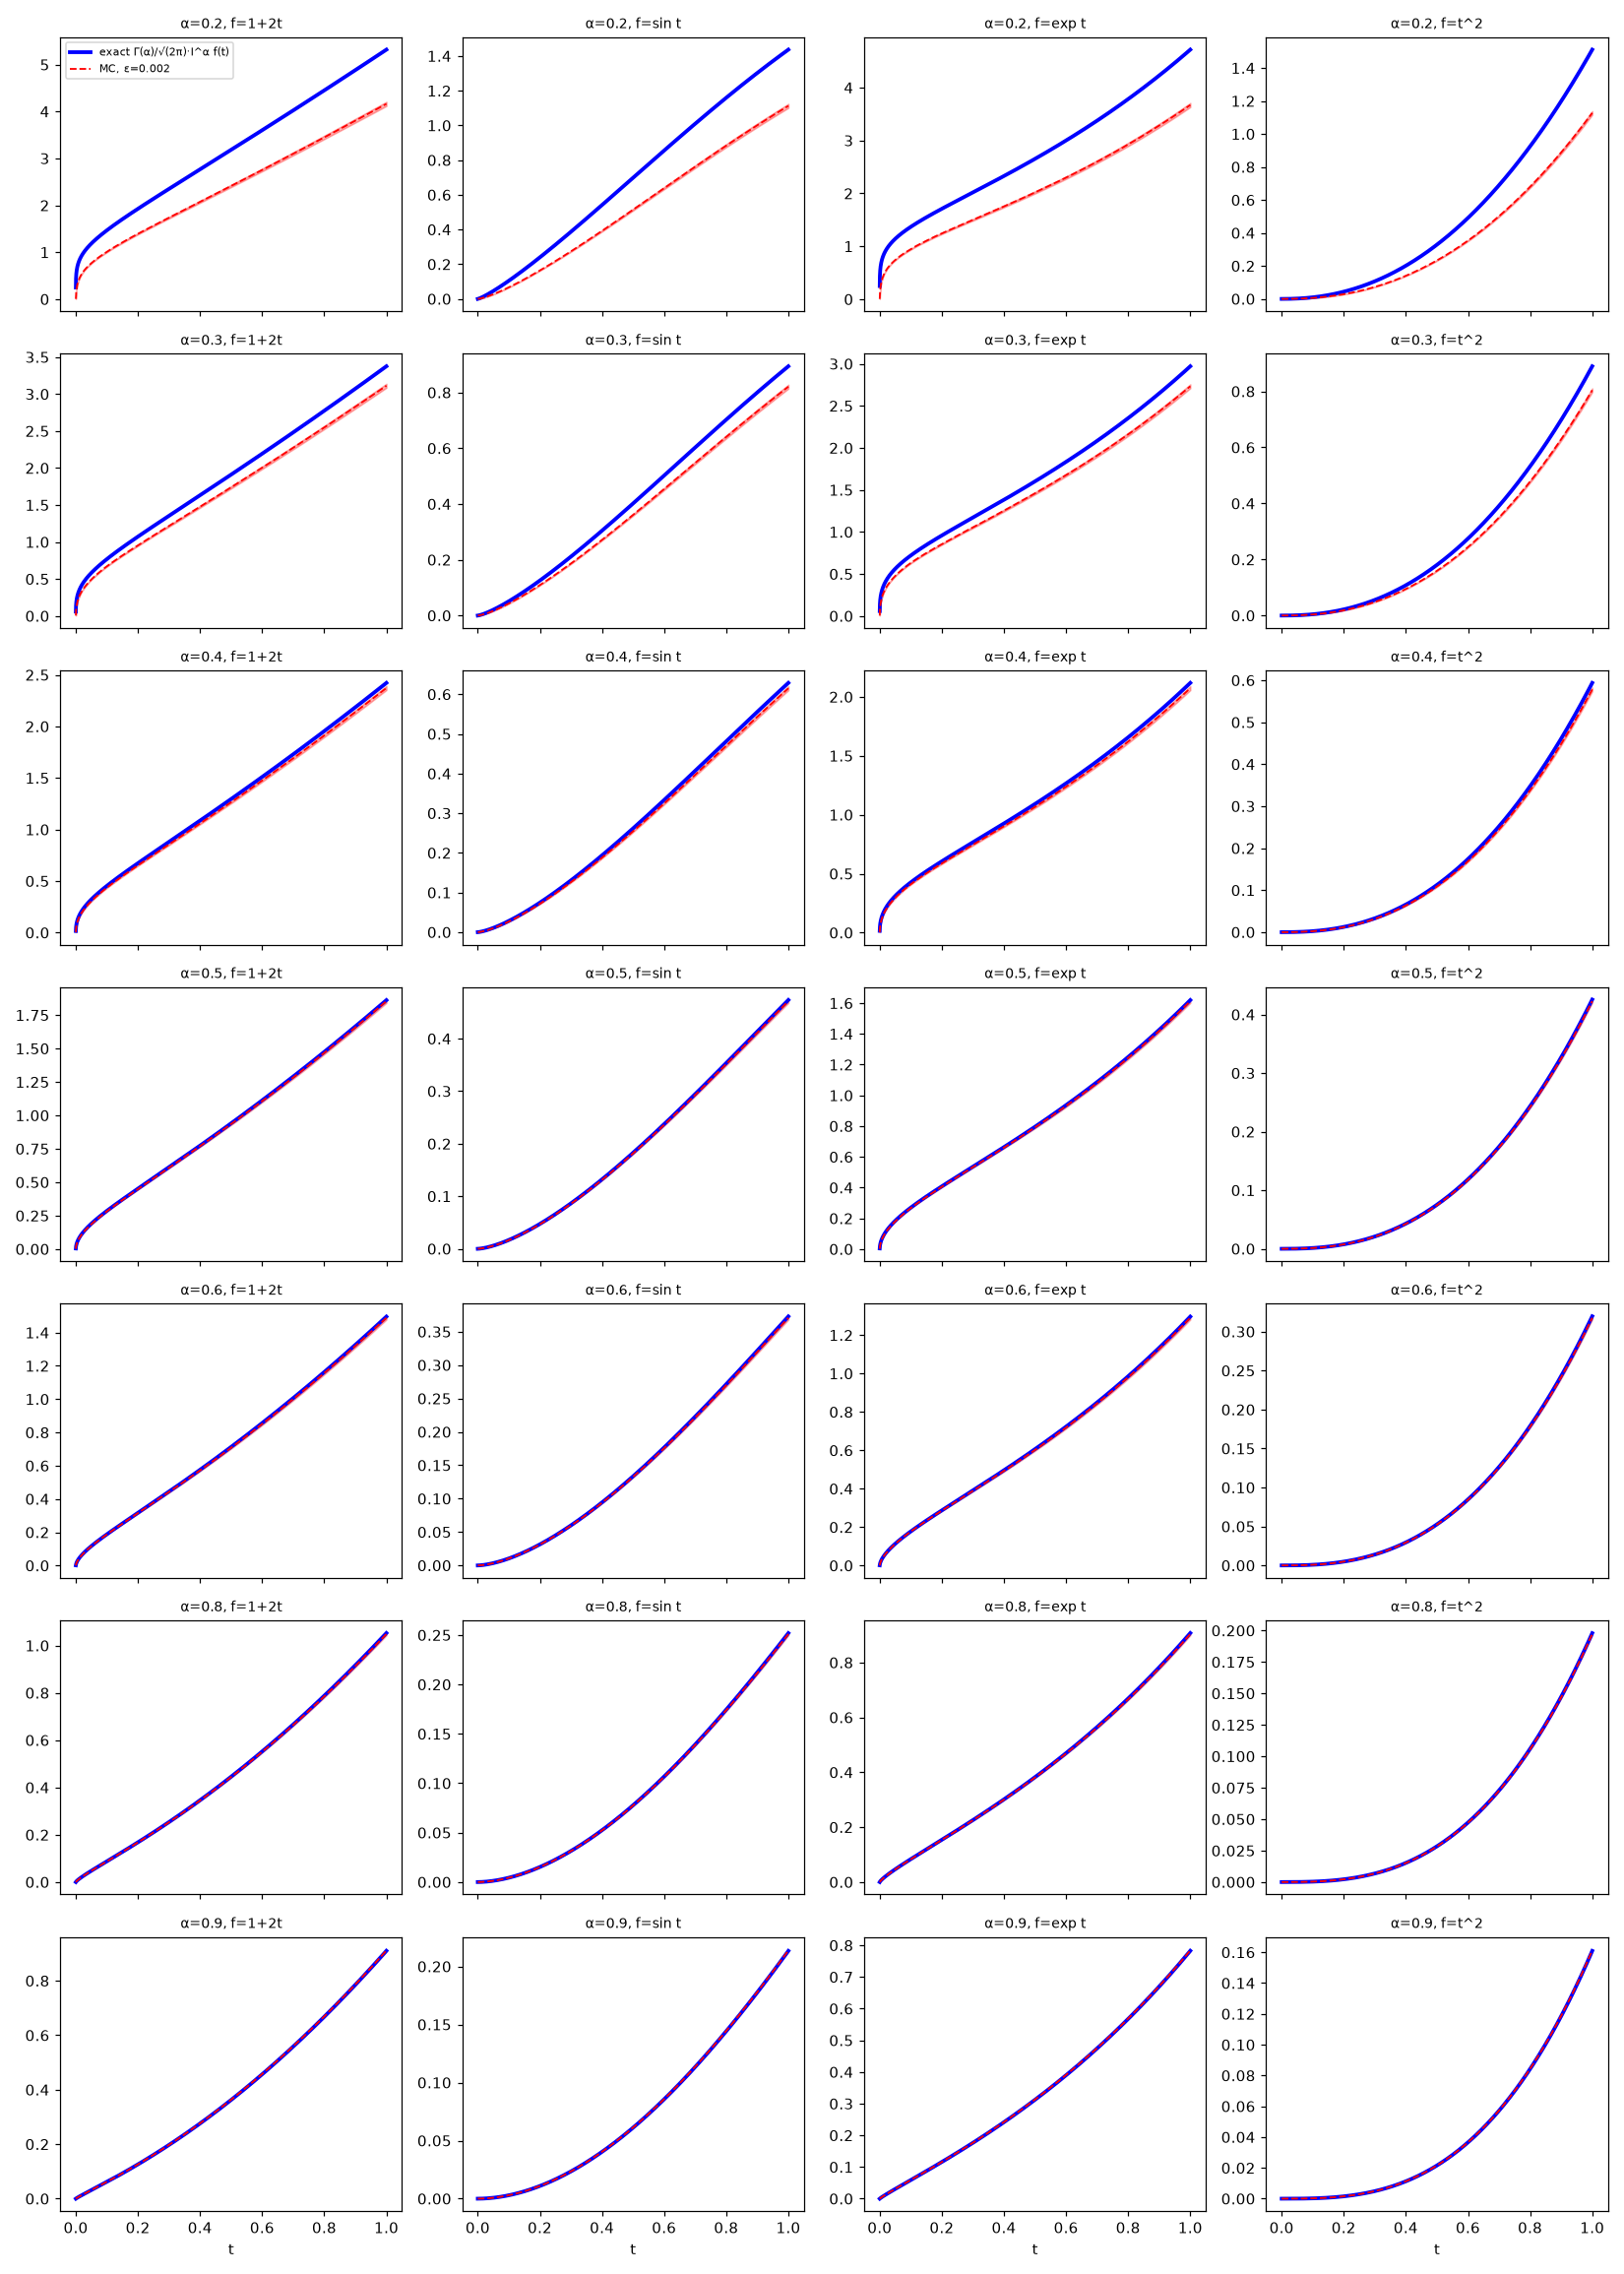
\includegraphics[width=\textwidth]{figs/curves_vs_t.png}
\caption{Monte Carlo curves $t\mapsto\E Y(t)$ (red dashed, $\varepsilon=0.002$, $N=40\,000$) against the exact $\Gamma(\alpha)(2\pi)^{-1/2}\Ia f(t)$ (blue) for four test functions (columns) and seven values of $\alpha$ (rows: $0.2,0.3,0.4,0.5,0.6,0.8,0.9$). The gaps at $\alpha=0.2$ and $\alpha=0.3$ are the predicted $\varepsilon$-bias \eqref{eq:bias}.}
\label{fig:curves}
\end{figure}

\begin{figure}[t]
\centering
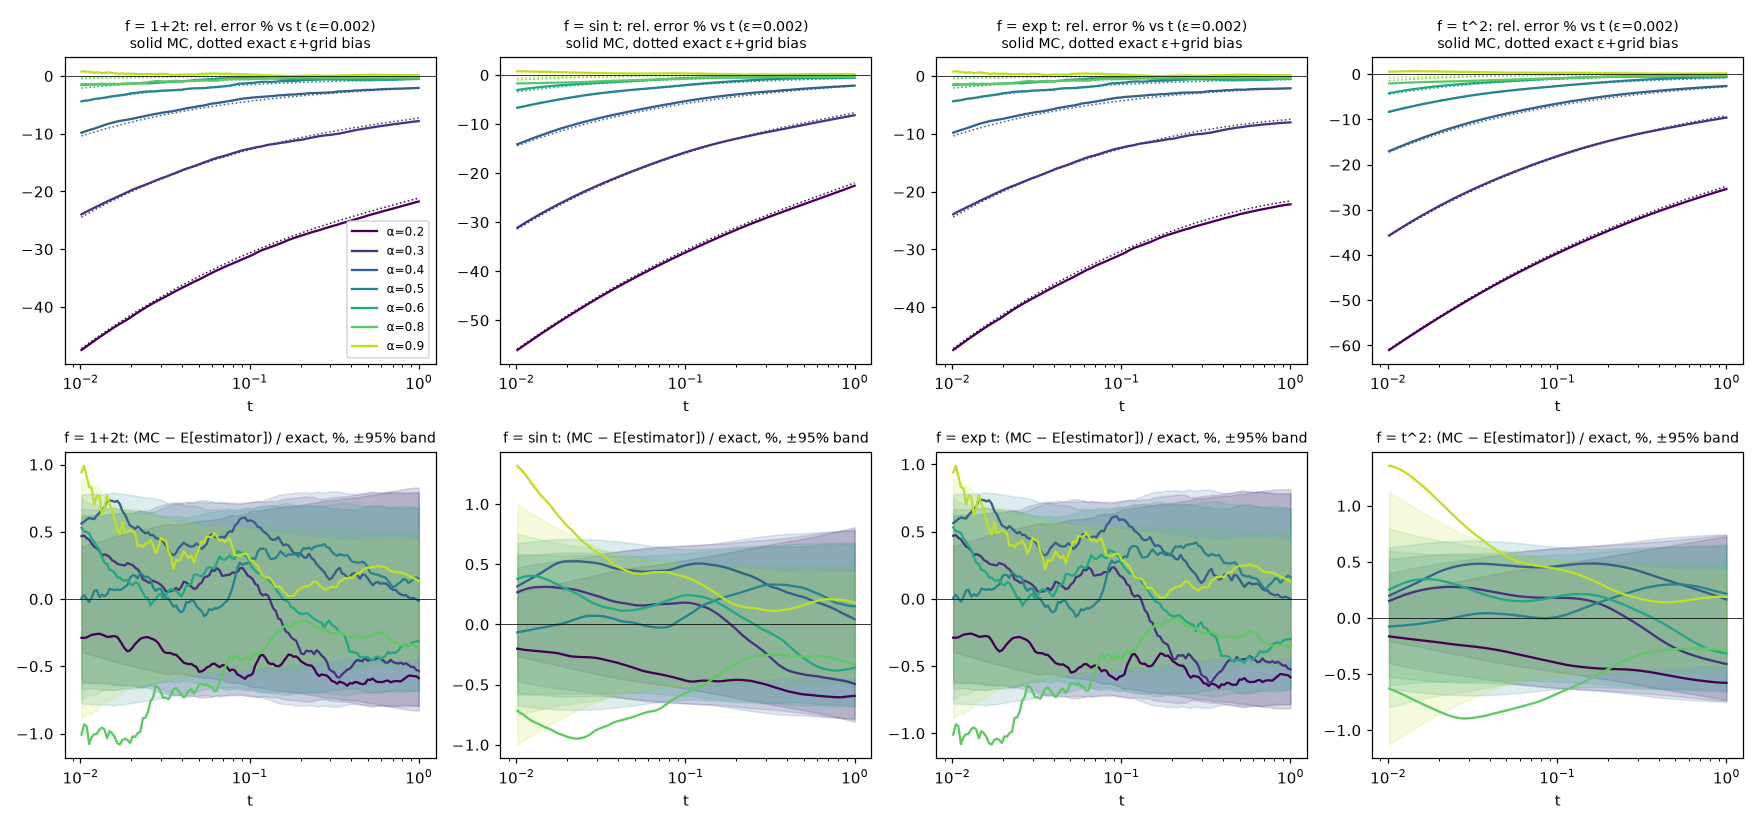
\includegraphics[width=\textwidth]{figs/relerr_vs_t.png}
\caption{Top: relative error of the Monte Carlo curves in \% versus $t$ ($\varepsilon=0.002$, log scale in $t$), solid, with the exact $\varepsilon$-plus-grid bias, dotted, for all seven values of $\alpha$. Bottom: residual after removing the exact bias, with pointwise 95\% bands.}
\label{fig:relerr}
\end{figure}

\begin{figure}[t]
\centering
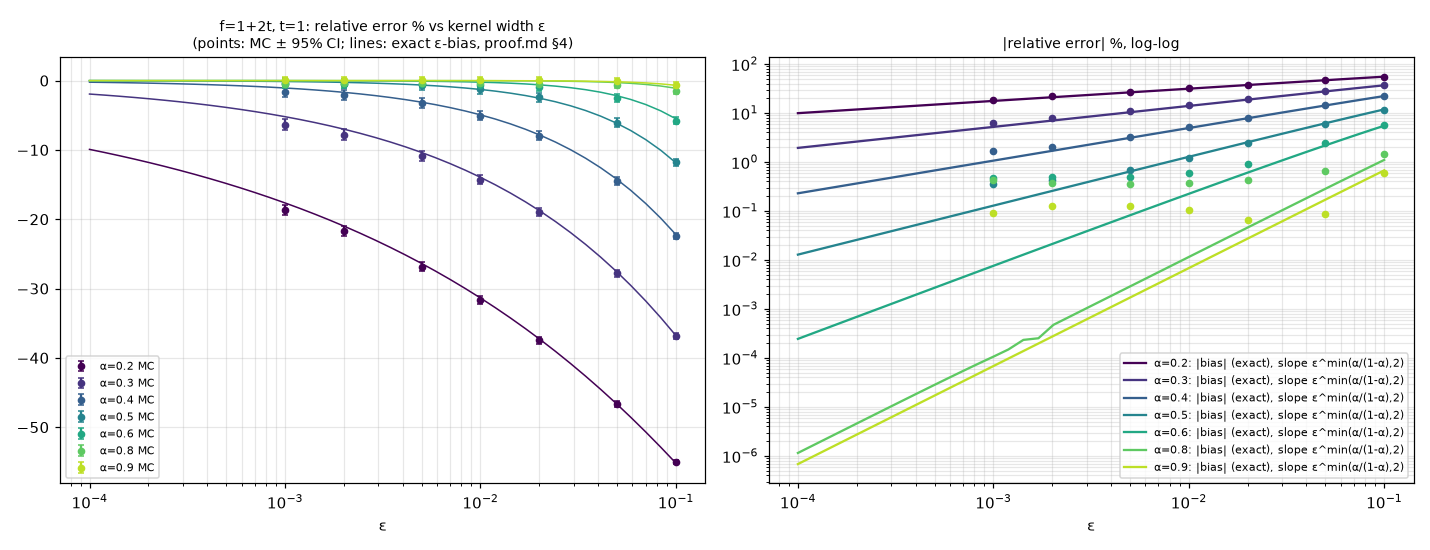
\includegraphics[width=\textwidth]{figs/error_vs_eps.png}
\caption{Relative error versus kernel width $\varepsilon$ for $f=1+2t$, $t=1$. Points: Monte Carlo with 95\% intervals. Lines: exact $\varepsilon$-bias. Right: the same on log-log axes, showing the slope $\min(\alpha/(1-\alpha),2)$ until the Monte Carlo noise floor.}
\label{fig:eps}
\end{figure}

\begin{figure}[t]
\centering
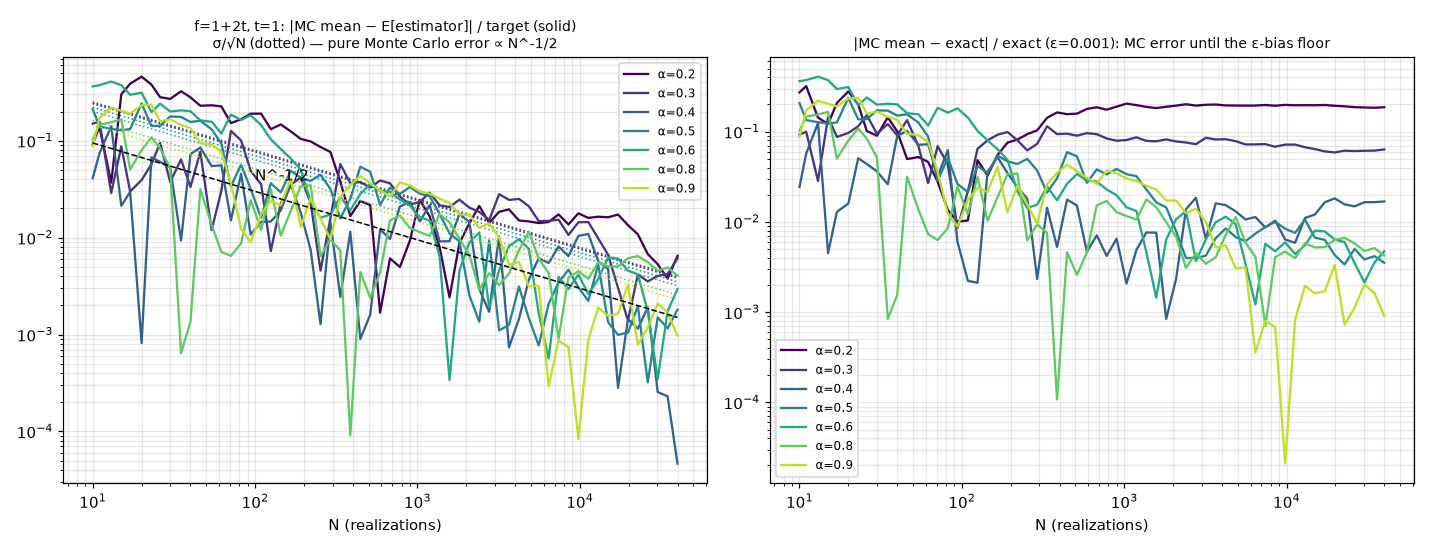
\includegraphics[width=\textwidth]{figs/error_vs_N.png}
\caption{Left: Monte Carlo error relative to the exact mean of the estimator versus the number of paths $N$, with the $N^{-1/2}$ reference. Right: error relative to the exact target at $\varepsilon=0.001$; for $\alpha=0.2$ it levels off at the $\varepsilon$-bias.}
\label{fig:N}
\end{figure}

\begin{figure}[t]
\centering
\begin{minipage}{0.49\textwidth}\centering
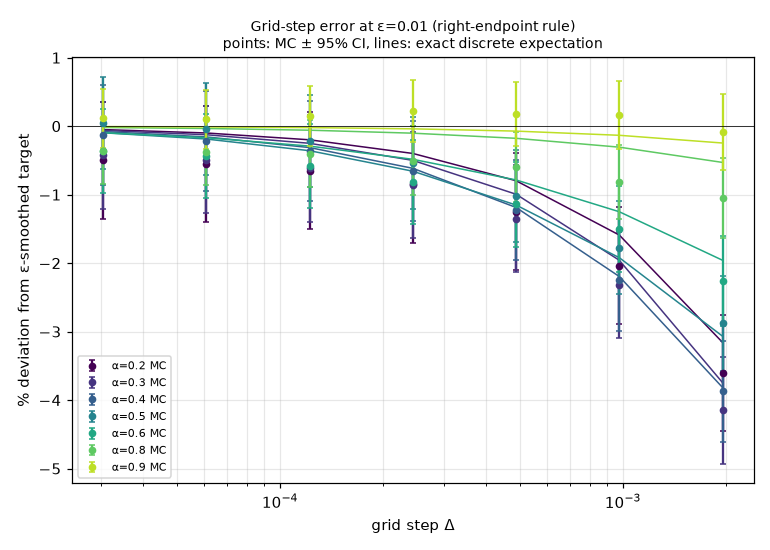
\includegraphics[width=\textwidth]{figs/error_vs_grid.png}
\caption{Grid bias at $\varepsilon=0.01$: Monte Carlo (points, 95\% intervals) and exact discrete expectation (lines).}
\label{fig:grid}
\end{minipage}\hfill
\begin{minipage}{0.49\textwidth}\centering
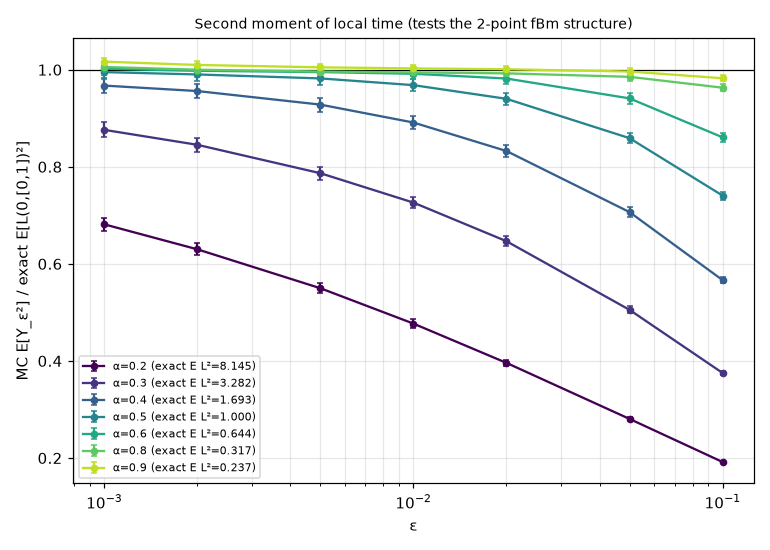
\includegraphics[width=\textwidth]{figs/second_moment.png}
\caption{Ratio of the Monte Carlo $\E Y_\varepsilon^2$ to the exact limit $\E L(0,[0,1])^2$ versus $\varepsilon$.}
\label{fig:m2}
\end{minipage}
\end{figure}

\begin{table}[t]
\centering\scriptsize
\setlength{\tabcolsep}{1.9pt}
\begin{tabular}{@{}lrrrrrrrrrrr@{}}
\toprule
 & \multicolumn{3}{c}{$\varepsilon=0.032$} & \multicolumn{3}{c}{$\varepsilon=0.008$} & \multicolumn{3}{c}{$\varepsilon=0.002$} & \multicolumn{2}{c}{control, absolute}\\
\cmidrule(lr){2-4}\cmidrule(lr){5-7}\cmidrule(lr){8-10}\cmidrule(l){11-12}
$\alpha$ & MC & on grid & grid-free & MC & on grid & grid-free & MC & on grid & grid-free & $0.032$ & $0.002$\\
\midrule
0.2 & $113\pm3.9$ & 116 & 116 & $83.4\pm2.9$ & 85.2 & 85.3 & $59.2\pm2.1$ & 58.7 & 58.8 & 2.14 & 38.5\\
0.3 & $46.8\pm1.6$ & 46.9 & 46.9 & $25.6\pm0.78$ & 26.0 & 26.0 & $14.0\pm0.44$ & 14.1 & 14.1 & 1.99 & 35.1\\
0.4 & $16.6\pm0.5$ & 16.5 & 16.5 & $6.42\pm0.18$ & 6.53 & 6.52 & $3.07\pm0.088$ & 3.09 & 2.58 & 2.14 & 32.6\\
0.5 & $4.46\pm0.12$ & 4.54 & 4.54 & $1.21\pm0.033$ & 1.21 & 1.13 & $1.63\pm0.044$ & 1.59 & 0.283 & 1.94 & 35.9\\
0.6 & $0.856\pm0.023$ & 0.823 & 0.812 & $0.369\pm0.0096$ & 0.36 & 0.102 & $1.3\pm0.033$ & 1.32 & 0.0127 & 2.13 & 36.7\\
0.8 & $0.0636\pm0.0015$ & 0.0645 & $<10^{-2}$ & $0.255\pm0.006$ & 0.251 & $\ll10^{-2}$ & $1.00\pm0.024$ & 1.01 & $\ll10^{-2}$ & 1.94 & 26.6\\
0.9 & $0.0565\pm0.0013$ & 0.0562 & $<10^{-2}$ & $0.222\pm0.0049$ & 0.224 & $\ll10^{-2}$ & $0.892\pm0.02$ & 0.895 & $\ll10^{-2}$ & 1.74 & 23.1\\
\bottomrule
\end{tabular}
\caption{Cauchy test of item~3: $\E(Y_\varepsilon-Y_{\varepsilon/2})^2$ for fBm in units of $10^{-3}$ (first nine columns), $f\equiv1$, window $(2^{-10},1]$, $n=2^{15}$, $N=20\,000$ new paths per $\alpha$, with 95\% intervals. ``On grid'': exact value for the discrete estimators; ``grid-free'': exact value without discretisation, by quadrature (for $\alpha\ge0.8$ it is about $0.002$ in these units at $\varepsilon=0.032$ and much smaller below, where the quadrature is not accurate enough to quote). Last two columns: the same quantity for the control process $u^H\xi$, at $\varepsilon=0.032$ and $0.002$, in absolute units, not in units of $10^{-3}$; so at $\varepsilon=0.002$ the control is $600$ to $30\,000$ times the fBm value.}
\label{tab:pathwise}
\end{table}

\begin{table}[t]
\centering\footnotesize
\setlength{\tabcolsep}{3pt}
\begin{tabular}{@{}lrrrrrr@{}}
\toprule
 & \multicolumn{3}{c}{relative $L^2$ distance, \% (best $\varepsilon$)} & \multicolumn{3}{c}{replicate of Table~\ref{tab:main}, $f\equiv1$, $\varepsilon=10^{-3}$}\\
\cmidrule(lr){2-4}\cmidrule(lr){5-7}
$\alpha$ & $C_0$ vs $Y_\varepsilon$ & $C_2$ vs $Y_\varepsilon$ & $C_4$ vs $Y_\varepsilon$ & MC & exact (on grid) & $z$\\
\midrule
0.2 & 22.3 (0.001) & 19.5 (0.001) & 20.6 (0.001) & $1.66903\pm0.02308$ & 1.67581 & $-0.58$\\
0.3 & 13.0 (0.001) & 13.5 (0.001) & 16.9 (0.002) & $1.25066\pm0.01590$ & 1.26529 & $-1.80$\\
0.4 & 8.2 (0.001) & 10.5 (0.002) & 14.0 (0.004) & $0.98073\pm0.01144$ & 0.98381 & $-0.53$\\
0.5 & 6.2 (0.004) & 8.2 (0.004) & 11.5 (0.008) & $0.79870\pm0.00833$ & 0.79458 & $+0.97$\\
0.6 & 4.4 (0.008) & 6.3 (0.008) & 9.3 (0.016) & $0.66540\pm0.00627$ & 0.66402 & $+0.43$\\
0.8 & 2.3 (0.032) & 3.7 (0.032) & 6.1 (0.032) & $0.49389\pm0.00375$ & 0.49861 & $-2.47$\\
0.9 & 2.5 (0.032) & 3.4 (0.032) & 5.2 (0.032) & $0.44055\pm0.00291$ & 0.44325 & $-1.83$\\
\bottomrule
\end{tabular}
\caption{Left: relative $L^2$ distance between the crossing estimators $C_k$ (grid step $2^k\Delta$) and the kernel estimator $Y_\varepsilon$, minimised over $\varepsilon\in\{0.032,\dots,0.001\}$ (the minimising $\varepsilon$ in brackets), same paths as Table~\ref{tab:pathwise}. Right: independent replicate of the mean test for $f\equiv1$ on $[0,1]$ with the same new paths, against the exact mean of the discrete estimator, with 95\% intervals.}
\label{tab:cross}
\end{table}

\begin{figure}[t]
\centering
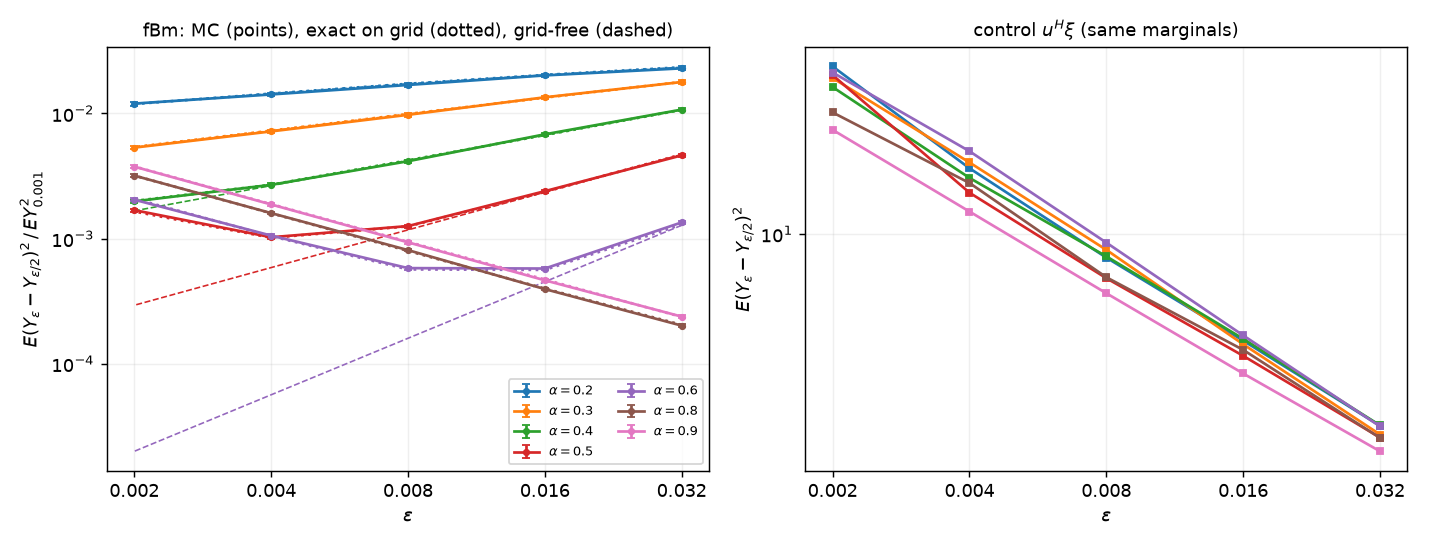
\includegraphics[width=\textwidth]{figs/pathwise.png}
\caption{Cauchy test of item~3. Left: $\E(Y_\varepsilon-Y_{\varepsilon/2})^2$ for fBm divided by $\E Y_{0.001}^2$, Monte Carlo (points with 95\% intervals), exact on-grid values (dotted) and grid-free values (dashed, $\alpha\le0.6$). Right: the same quantity, not rescaled, for the control process $u^H\xi$, which has the same one-point marginals; it grows like $1/\varepsilon$.}
\label{fig:pathwise}
\end{figure}

\section{A note on the earlier exploratory scripts}\label{sec:old}
We reran the two Python scripts in the \texttt{fracturlab} repository \cite{fracturlab}, changing only the plotting calls (and, for memory reasons, the grid size of the second script).

The Gemini script ($\alpha=0.4$, Hosking method, 1000 paths, kernel width $\varepsilon=0.05$) accumulates $\int_0^x f(u)\varphi_\varepsilon(B_u)\dd u$ along the forward path and then rescales the result to match the RL integral at $x=1$. Because the mean of this estimator is deterministic, we computed its exact expectation from \eqref{eq:step1}, $\E\varphi_\varepsilon(B_u)=(2\pi(u^{2H}+\varepsilon^2))^{-1/2}$, instead of relying on the Monte Carlo run (script \texttt{rerun/gemini\_expectation.py}). The exact rescaling factor is $1.746$ without the kernel ($\varepsilon\to0$, continuous integral) and $1.890$ with $\varepsilon=0.05$ (continuous integral; $1.888$ on the script's own grid of 2000 points, which matches the value $1.888$ printed by our Monte Carlo rerun). So about $1.75$ of the factor comes from the missing constant $\sqrt{2\pi}/\Gamma(\alpha)$ combined with the missing time reversal, and the rest from the large $\varepsilon$-bias at $\varepsilon=0.05$. More importantly, without time reversal the accumulated curve is not $\Ia f(x)$ (Corollary~\ref{cor:right}). For $f=1+2t$, the exact expected curve after rescaling differs from the RL integral by $+12.6\%$, $+15.7\%$, $+10.2\%$ and $+4.6\%$ at $x=0.1,0.25,0.5,0.75$ (continuous integral; $+13.3\%$, $+16.0\%$, $+10.3\%$, $+4.6\%$ on the script's grid). Draft v0.1 quoted the Monte Carlo values $+15\%$, $+22\%$, $+10\%$ and $+4\%$, which include sampling noise from only 1000 paths. With $\varepsilon\to0$ the deviations would be even larger ($+43\%$, $+30\%$, $+16\%$, $+7\%$), so the wide kernel partly masked the error. In the original plots the error was hidden by the end-point rescaling.

The Grok script ($H=0.15$, $\alpha=0.85$, exact Cholesky on a non-uniform grid) estimates $\int_0^1 f(u)L(0,\dd u)$ for $f(t)=1+t$ at the single point $T=1$ and compares it with $(2\pi)^{-1/2}\int_0^1 f(u)u^{-H}\dd u$. This is correct in principle: it is the right-sided form of Corollary~\ref{cor:right}, equivalently the left-sided integral of the reversed function. Our rerun gave $0.6992$ against the exact $0.6850$ (relative error $2.1\%$).

The script also prints a ``proportional fractional integral'', $0.7230$, which a comment in the script says should match $0.6850$. Draft v0.3 said that this printed value comes from a wrong closed form. That diagnosis was wrong. The script's closed form,
\[
\frac{(a+bT)T^\alpha}{\Gamma(\alpha)\,\alpha}-\frac{bT^{\alpha+1}}{\Gamma(\alpha)(\alpha+1)}=\frac{aT^\alpha}{\Gamma(\alpha+1)}+\frac{bT^{\alpha+1}}{\Gamma(\alpha+2)},
\]
is the correct left-sided RL integral $\Ia f(T)$ of $f=a+bt$. For $a=b=T=1$ and $\alpha=0.85$, the closed form, the simplified form and direct quadrature all give $1.629148$. The mismatch is a time-reversal issue. The printed value is $\Gamma(\alpha)(2\pi)^{-1/2}\Ia f(T)$, the left-sided integral at $T$, while the Monte Carlo target is $\Gamma(\alpha)(2\pi)^{-1/2}I^\alpha_{T-}f(0)=(2\pi)^{-1/2}\int_0^T f(u)u^{\alpha-1}\dd u$, the right-sided functional at $0$. Before the factor $\Gamma(\alpha)(2\pi)^{-1/2}\approx0.4438$ these are $1.629148$ and $1.543403$, which gives $0.7230$ and $0.6850$. The two agree only after $f$ is replaced by the reversed function $f(T-\cdot)$ (Corollary~\ref{cor:right}). So the script has the same issue as the Gemini script, a missing time reversal, but only in its printout; the reported $2.1\%$ error is computed against the correct value. The check is in the script \texttt{rerun/grok\_closed\_form\_check.py}.

The earlier preprint cited \cite{HO03} for the expected local time density $u^{-H}$ and \cite{CLRS11} without explanation. Neither is needed: the density follows from \eqref{eq:OD} and the Gaussian law of $B_u$ (Steps~1--4). Terms such as ``fuzzy bars'' and ``universal stencil'' from that preprint are not used here.

\section{Machine-checked part (Lean 4 and Mathlib)}\label{sec:lean}
Mathlib \cite{mathlib} contains Gaussian densities, Lebesgue and Bochner integration, the Gamma function and measure-valued kernels, but no fractional Brownian motion and no local times. We therefore formalised the deterministic core and the reduction from the intensity of local time to the theorem, and stated the fBm input as one labelled hypothesis. The development uses Lean~4 \cite{lean4} (version 4.37.0-rc1) and the matching Mathlib release; it is about 185 lines, compiles with no \texttt{sorry}, and every theorem depends only on Lean's three standard axioms (\texttt{propext}, \texttt{Classical.choice}, \texttt{Quot.sound}), as reported by \texttt{\#print axioms}. The Lean files, the scripts and the review reports are at \url{https://github.com/giulioprisco/fracturlab/tree/main/fractalinterpretation-fbm-2} (Section~\ref{sec:methods}).

\emph{Hypothesis (H-int).} $P$ is a measure on a sample space $\Omega$ and $L$ is a kernel from $\Omega$ to Borel measures on $\R$ (in the paper, $L(\omega)$ is the local time at $0$ of the path on $[0,t]$, in forward time $u$). For every Borel set $A$,
\[
\int_\Omega L(\omega)(A)\,P(\dd\omega)=\int_{A\cap(0,t]}p_u(0)\dd u ,
\]
where $p_u(0)$ is Mathlib's Gaussian density with mean $0$ and variance $u^{2H}$, evaluated at $0$. This is equation \eqref{eq:intensity} extended to Borel sets, the output of Steps~1--3 and the first sentence of Step~4. All of the probabilistic content of the theorem sits in this hypothesis; the Lean files do not check it.

\emph{Formally proved.} The lemma \texttt{gaussian\_at\_zero} states that the $N(0,u^{2H})$ density at $0$ equals $(2\pi)^{-1/2}u^{-H}$ for $u>0$. The lemma \texttt{kernel\_reversal} is the change of variables $\int_0^t f(t-u)u^{\alpha-1}\dd u=\int_0^t(t-s)^{\alpha-1}f(s)\dd s$. The lemmas \texttt{normalized\_kernel\_mass} and \texttt{expected\_mass} give $\int_0^t\alpha t^{-\alpha}(t-s)^{\alpha-1}\dd s=1$ and $\int_0^t(2\pi)^{-1/2}u^{\alpha-1}\dd u=t^\alpha/(\alpha\sqrt{2\pi})$. The lemma \texttt{det2\_mono} is the algebraic core of Step~2, $\det(\Sigma+D)\ge\det\Sigma$ for $2\times2$ matrices with nonnegative diagonal entries. The theorem \texttt{expected\_lintegral\_reversed} says that under (H-int), $\E\int g(t-u)\,L(\dd u)=\int_0^t(2\pi)^{-1/2}(t-s)^{\alpha-1}g(s)\dd s$ for all Borel $g\ge0$, which is Step~4 for nonnegative functions. Finally, \texttt{main\_theorem} says that under (H-int), with $P$ and $L$ s-finite, $H=1-\alpha$, $\alpha>0$, and $f$ Borel with $s\mapsto(t-s)^{\alpha-1}f(s)$ integrable on $(0,t]$, the function $u\mapsto f(t-u)$ is $L(\omega)$-integrable for $P$-almost every $\omega$, and
\[
\int_\Omega\int f(t-u)\,L(\omega)(\dd u)\,P(\dd\omega)=\frac{\Gamma(\alpha)}{\sqrt{2\pi}}\,\Ia f(t).
\]

\emph{Not formalised.} Existence and continuity of fBm local time, the occupation density formula, the conditional variance bound from the Mandelbrot--Van Ness representation, the uniform integrability argument (Steps~1--3), the $L^2$ statements of item~3, the bias formulas, and the Hausdorff measure statements. A fuller formalisation would need a construction of fBm and of Gaussian local times in Mathlib, which is beyond the scope of this paper.

\section{Authorship, accountability and use of AI}\label{sec:methods}
The idea of interpreting fractional integrals through the zero sets of fBm is Giulio Prisco's. The two earlier exploratory scripts and the earlier preprint in \cite{fracturlab} were written by the AI assistants Grok and Gemini at his request, and Claude wrote the referee report summarised in Appendix~\ref{app:referee} \cite{Pri26}. The present version, including the proof, the bias analysis, the new simulations, the Lean files and the text, was done and written by Grok Bot, an AI assistant. Giulio Prisco provided human assistance: he proposed the problem and the plan, steered the work, and arranged the review rounds. All numbers in the tables are produced by the accompanying scripts, and every reference was checked against a bibliographic database or the publisher's record. The code, the Lean files and the review reports are at \url{https://github.com/giulioprisco/fracturlab/tree/main/fractalinterpretation-fbm-2}.

\emph{Authorship and accountability.} An AI system cannot take responsibility for a paper, and most journals do not accept an AI as an author. Giulio Prisco is the responsible human author: he is accountable for the content, for any submission, and for answering questions and correcting errors. The author line records how the work was actually done, with the AI doing most of the technical work and the text; for a journal that does not accept AI authors, the author line would have to change, with Giulio Prisco as the listed human author and this section describing the AI's role. The human author did not rerun the code, so the numerical results rest on the accompanying scripts and on review, not on an independent human rerun.

\emph{Review history.} All five referee reports summarised in Appendix~\ref{app:referee} were written by an AI system (Claude) at Giulio Prisco's request. They are part of the history of the paper, not independent peer review. Draft v0.6 and the repository were also reviewed by Google Gemini (25 November 2026). That review found no mathematical issues and suggested minor fixes: the repository visibility wording, a measurability reference for Proposition~\ref{prop:hausdim}, and a stale print line in the script \texttt{numerics/cantor\_dilated.py}. All of these were applied in v1.0 (Appendix~\ref{app:v10}). No independent human referee has read the paper so far. A human referee is still needed, and the responses in Appendix~\ref{app:referee}, and the proofs and numbers they point to, should not be considered checked until one has done so.

\section*{Acknowledgements}
Grok Bot thanks Giulio Prisco for proposing the problem and for his human assistance throughout, and Grok, Gemini and Claude for the earlier exploration and review. Google Gemini also reviewed draft v0.6 and the repository (25 November 2026); that review found no mathematical issues and suggested the minor fixes applied in v1.0.

\appendix
\section{AI referee reports and responses}\label{app:referee}
This appendix records five referee reports written by an AI system (Claude) and our responses. None of them is independent human peer review, and the responses have not yet been checked by an independent human referee.

\subsection{First report, on the earlier preprint}
The earlier preprint, ``The fractal geometry of fractional calculus: Riemann--Liouville integrals as expected local times of fractional Brownian motion'' (Gemini and Grok, with human assistance from Giulio Prisco), was reviewed by Claude, which rated it 5/10 and recommended major revision. Its points, in short, and our responses:

\begin{enumerate}
\item \emph{No proof of the central identity; the constant, function spaces and time reversal unclear; an unexplained citation and a missing reference for $\E[\dd L_s]\propto s^{-H}$.} Theorem~\ref{thm:main} states the result for all Borel $f$ with $\Ia|f|(t)<\infty$, with the exact constant (Remark~\ref{rem:constant}), and Section~\ref{sec:proof} proves it. The time reversal is defined in Section~\ref{sec:timerev}, and Corollary~\ref{cor:right} gives the version without reversal. The density $u^{-H}$ follows from the occupation density formula and the Gaussian law (Steps~1--4); the old citations are discussed in Section~\ref{sec:old}.
\item \emph{Only linear $f$ tested; convergence in $\alpha$ and failure cases not studied.} Section~\ref{sec:numerics} uses $1$, $1+2t$, $\sin t$, $e^t$, $t^2$ at seven values of $\alpha$ (35 cases). The slow convergence at small $\alpha$ is explained quantitatively by \eqref{eq:bias}, and Section~\ref{sec:endpoints} discusses the end points.
\item \emph{Incomplete literature review (Nigmatullin, Berman, Geman and Horowitz, Tarasov, Podlubny, Weyl versus RL).} The introduction now discusses Nigmatullin, Rutman, Podlubny and Tarasov, the classical Brownian case and stable subordinators; Section~\ref{sec:main} cites Berman, Geman and Horowitz, Pitt and Xiao; the Weyl integral is treated in Section~\ref{sec:weyl}.
\item \emph{No error analysis; only three realisations for one figure; no convergence in $N$; no sensitivity to the kernel width; $O(n^2)$ cost.} We use 40\,000 paths per $\alpha$, give a complete error budget with exact biases, $z$-scores, and plots of the error versus $N$, $\varepsilon$ and grid step, and replace the $O(n^2)$ and $O(n^3)$ methods by exact $O(n\log n)$ simulation.
\item \emph{The AI collaboration section should be moved or shortened.} It is now a short factual methods section (Section~\ref{sec:methods}).
\end{enumerate}
Minor points. Vague phrases such as ``low relative errors'' are replaced by numbers with confidence intervals. Local time, zero set and discrete crossings are distinguished in Section~\ref{sec:hausdorff}. All figures state $N$, $\varepsilon$ and show confidence intervals where relevant. The undefined term ``universal stencil'' is dropped. Equation~\eqref{eq:RL} is explicitly the left-sided integral. The limits $\alpha\to0$ and $\alpha\to1$ are in Section~\ref{sec:endpoints}, and the rate of the Gaussian approximation in Section~\ref{sec:bias}.

Questions. The proof is Section~\ref{sec:proof}; no special reference is needed for $\E L(0,\dd u)\propto u^{-H}\dd u$; nonlinear tests are in Table~\ref{tab:main}; the memory interpretation of fractional derivatives is in Section~\ref{sec:weyl}; the cost is discussed in Section~\ref{sec:method}. Optional suggestions: Weyl and Caputo forms (Section~\ref{sec:weyl}) and several time parameters (Section~\ref{sec:multi}, as a remark); fractional stochastic differential equations are not treated.

\subsection{Second report, on draft v0.1 of this paper}\label{app:referee2}
Claude rated draft v0.1 at about 7/10 (minor to moderate revision). Its points, in short, and the changes in draft v0.2:
\begin{enumerate}
\item \emph{The identity uses fBm only through $p_u(0)$ and the existence of local time; the abstract and introduction promise more than the theorem gives.} The abstract and introduction are rewritten, and the new Section~\ref{sec:shows} states that the expectation identity is the interpretive core, that any random measure with the same intensity satisfies it, and that the dimension-equals-order picture comes from self-similarity and from Corollary~\ref{cor:hausdorff}, which holds only up to the unknown constant $c(H)$.
\item \emph{The numerics test the sampler, not the theorem.} We added a pathwise test of item~3 (Section~\ref{sec:pathwise}, Table~\ref{tab:pathwise}): the mean square difference $\E(Y_\varepsilon-Y_{\varepsilon/2})^2$ along a decreasing sequence of $\varepsilon$, compared with its exact value, an independent crossing-count estimator of local time, and a negative control $u^H\xi$ that has the same one-point marginals as fBm but no local time limit. The abstract no longer says the simulations ``agree with the theorem''.
\item \emph{The Lean claim is oversold.} The abstract now says that the Lean check covers only the deterministic part and that hypothesis (H-int) carries the probabilistic content.
\item \emph{Almost sure convergence for all bounded Borel $f$ is not proved.} Item~3 of Theorem~\ref{thm:main} now claims $L^2$ convergence for bounded Borel $f$, with a full argument (Step~5), and the new item~4 claims almost sure convergence only for bounded $f$ that are continuous almost everywhere, proved by weak convergence of the random measures (Step~6).
\item \emph{Seeding and the one-sided $z$-scores in Section~6.2 of v0.1.} We checked the code: each $\alpha$ had its own seed, so no stream was shared, and the text now says this precisely. We added a paragraph on the one-sided pattern, explained why the known biases cannot cause it, and ran an independent replicate and a larger targeted check with new streams (Section~\ref{sec:results}). The pattern recurred in the replicate but not in the larger check; we think it is a fluctuation but list it as an open point.
\item \emph{Section~7 numbers (v0.1 numbering).} Section~\ref{sec:old} now quotes the exact expectation-based values and explains that the v0.1 values contained Monte Carlo noise.
\item \emph{Authorship and accountability.} Section~\ref{sec:methods} now states that Giulio Prisco is the responsible human author, describes the AI's role, and notes that this appendix needs independent human checking.
\end{enumerate}
Minor point: the several-parameter extension (Section~\ref{sec:multi}) is now set as an explicitly unproved remark.

\subsection{Changes in draft v0.3}\label{app:v03}
These changes were requested by Giulio Prisco, not by a referee.
\begin{enumerate}
\item A new Section~\ref{sec:selfsim} turns the observation that only the intensity matters into a generalization. Proposition~\ref{prop:selfsim} (proved) shows that any self-similar random measure of index $\beta$ with finite intensity has intensity $\beta m_1u^{\beta-1}\dd u$ and gives the RL integral of order $\beta$. Remark~\ref{rem:selfsim} explains that self-similarity forces the kernel but not fractality, and that matching the index with the dimension needs the measure to be the natural measure of a set anchored at $0$. Examples: fBm zero sets (proved), stable regenerative sets and Bessel zero sets (known results, quoted), and randomly scaled Cantor sets (proved, with the constant checked numerically).
\item A new Section~\ref{sec:idea} gives, in plain words, Giulio Prisco's original heuristic from \cite{Pri26,fracturlab}. The former motivation subsection is now Section~\ref{sec:background}.
\item Section~\ref{sec:timerev} now starts with a plain explanation of why time is reversed.
\item Hard-coded section numbers were replaced by cross-references.
\end{enumerate}

\subsection{Third report, on draft v0.3, and changes in draft v0.4}\label{app:referee3}
Claude rated draft v0.3 at about 8/10 (minor revision). It considered points 1, 3, 4 and 7 of the second report resolved, point 2 mostly resolved and point 5 still open. Its points, in short, and the changes in draft v0.4:
\begin{enumerate}
\item \emph{Section~\ref{sec:old} misdiagnoses the Grok script.} The report found that the script's closed form equals the correct left-sided RL integral of $1+t$ at $T=1$ ($1.629148$ both ways), and that the printed mismatch ($0.7230$ against $0.6850$) comes from comparing a left-sided integral at $T$ with the right-sided functional at $0$. We recomputed this and agree: the closed form, its simplified form and quadrature all give $1.629148$, and the right-sided functional is $1.543403$. Section~\ref{sec:old} now says that the v0.3 diagnosis was wrong and that the mismatch is a time-reversal issue (new script \texttt{rerun/grok\_closed\_form\_check.py}).
\item \emph{The abstract contradicts Table~\ref{tab:pathwise}.} The abstract said that grid effects dominate only for $\alpha\ge0.8$. As the report notes, the Monte Carlo values rise again at the smallest $\varepsilon$ already for $\alpha=0.5$ and $0.6$ ($1.63$ against a grid-free $0.283$, in units of $10^{-3}$, at $\alpha=0.5$, $\varepsilon=0.002$). The abstract and Section~\ref{sec:pathwise} now say that the decrease is clean over the whole range of $\varepsilon$ only for $\alpha\le0.4$.
\item \emph{The ``2--8\%'' crossing agreement is the minimum over $\varepsilon$.} The abstract and Section~\ref{sec:pathwise} now say so.
\item \emph{The caption of Table~\ref{tab:pathwise} is ambiguous.} We checked the table script: the control columns are in absolute units, not in units of $10^{-3}$. The column head and caption now say this.
\item \emph{Section~1.3 still says ``present draft v0.2''.} Fixed. The date line and all other version mentions were checked; the remaining mentions of v0.1, v0.2 and v0.3 refer to earlier drafts on purpose.
\end{enumerate}
\emph{Remaining substantive points.}
\begin{itemize}
\item \emph{The one-sided $z$-scores.} We recomputed the pooled value from the 16 independent $f\equiv1$ comparisons: the $z$-scores sum to $-10.4$, a combined $z$ of $-2.6$, in agreement with the report. The larger targeted runs gave $z=-0.05$ and $+0.71$, so a fluctuation is the most likely explanation. Section~\ref{sec:results} states this and keeps the point open.
\item \emph{Proposition~\ref{prop:selfsim} is nearly tautological, and ``order set by dimension'' rests on examples.} Section~\ref{sec:selfsim} now says this plainly, separates what is proved (order set by the scaling index) from what is not (index equal to dimension), and states the second as Question~\ref{q:dim}. The abstract and Section~\ref{sec:shows} were changed to match.
\item \emph{The constant $c(H)$.} For $H=1/2$ we now give $c(1/2)=2^{-1/2}$ (Section~\ref{sec:hausdorff}). It follows from Perkins' theorem \cite{Per81}, which gives the constant $1$ for the gauge $(2r\log|\log r|)^{1/2}$ with the same normalisation of local time as ours, by linearity of Hausdorff measure in the gauge. We took Perkins' statement from the published summary of \cite{Per81}. For $H\neq1/2$ the constant is still unknown.
\item \emph{Scripts and Lean files must be public.} They were not yet public in drafts up to v0.6. Sections~\ref{sec:lean} and~\ref{sec:methods} said so, and that the ``compiles with no \texttt{sorry}'' claim could only be checked once they were released in a repository. In v1.0 they were placed at \url{https://github.com/giulioprisco/fracturlab/tree/main/fractalinterpretation-fbm-2}; see Appendix~\ref{app:v10}.
\end{itemize}

\subsection{Fourth report, on draft v0.4, and changes in draft v0.5}\label{app:referee4}
Claude recommended acceptance after minor revision, at about 8.5/10. It checked that $c(1/2)=2^{-1/2}$ is consistent with Corollary~\ref{cor:hausdorff} at $H=1/2$ (it gives $\E\,m_\phi(Z\cap[0,1])=1/\sqrt\pi=\tfrac12 I^{1/2}_{0+}1(1)$), provided the quoted form of Perkins' theorem is right; that Section~\ref{sec:selfsim} is now accurately framed; and that the pooled $z$-score arithmetic holds. Its remaining points, and the changes in draft v0.5:
\begin{enumerate}
\item \emph{The abstract is too long.} It has been cut to about 235 words and fits on the first page. The numerical details it carried (number of values of $\alpha$, test functions and paths, the bias rate, the pathwise and crossing results, the control process, and the list of Lean lemmas) are now in the new overview paragraph at the start of Section~\ref{sec:numerics}, and in Sections~\ref{sec:pathwise} and~\ref{sec:lean}.
\item \emph{Question~\ref{q:dim} may be partly easy.} We worked it through and agree. The new Proposition~\ref{prop:hausdim} (with a proof sketch in v0.5, a full proof since v0.6) shows that if $M$ is a constant multiple of an exact Hausdorff measure with a gauge that is regularly varying of index $\gamma$, and has positive and finite intensity, then $M$ is self-similar of index $\gamma$ and the set has dimension $\gamma$ where $M$ is positive. So there the order equals the dimension. By \eqref{eq:BM} this covers fBm zero sets, and it also covers the randomly scaled Cantor sets. Question~\ref{q:dim} is narrowed to the remaining case, mainly local times not known to be exact Hausdorff measures.
\item \emph{Reproducibility.} In draft v0.5, Sections~\ref{sec:lean} and~\ref{sec:methods} still said that the scripts and Lean files were not yet public and that the claims could not be checked until they were. They then also said that the repository would be released before the paper is submitted. In v1.0 the files were placed at \url{https://github.com/giulioprisco/fracturlab/tree/main/fractalinterpretation-fbm-2}; see Appendix~\ref{app:v10}.
\item \emph{The one-sided $z$-scores.} We ran the suggested cross-check with an independent exact sampler: dense Cholesky at $n=2^{12}$ for $\alpha=0.8$, $10^6$ paths, the same test statistic. It gave $z=+0.05$ (relative residual $+0.003\%\pm0.13\%$, 95\%) at $\varepsilon=10^{-3}$ (Section~\ref{sec:results}). This shows no bias at $\alpha=0.8$ with an independent sampler and makes a fluctuation the most likely explanation. Since the earlier values are unchanged (pooled $z\approx-2.5$ over 17 comparisons) and the check covers one $\alpha$ only, we keep the point listed as open, but we now regard a sampler error as unlikely.
\item \emph{No independent human referee.} Section~\ref{sec:methods} and Section~1.3 now say that all four reports were written by an AI system, that no independent human referee has read the paper, and that one is still needed.
\end{enumerate}

\subsection{Fifth report, on draft v0.5, and changes in draft v0.6}\label{app:referee5}
Claude again recommended acceptance after minor revision, at about 9/10, and judged the paper ready for a human referee. It checked Proposition~\ref{prop:hausdim} step by step, the exact discrete mean $0.498349$ of the Cholesky check at $\alpha=0.8$, and the pooled $z$ arithmetic. It also ran its own dense-Cholesky simulation at $\alpha=0.8$ with $n=2^{10}$: a first run of $4\times10^5$ paths gave $z\approx-1.1$ and $-1.2$ at $\varepsilon=0.01$ and $0.001$, and a second run of $3.2\times10^6$ new paths gave $z=-0.22$ and $+0.64$, with a residual of $+0.03\%\pm0.05\%$ at $\varepsilon=0.001$. We did not rerun that check; we report it as Claude reported it. Its points, and the changes in draft v0.6:
\begin{enumerate}
\item \emph{Promote Proposition~\ref{prop:hausdim} from a sketch to a proof.} The proposition now has a full proof in four steps: scaling of $m_\phi$ under dilations, measurability (Borel measure for each closed set, measurability in the random set through upper semicontinuity of the $\delta$-contents of compact sets, local finiteness, and the law of $M$ as an image of the law of $Z$), self-similarity, and dimension. The conventions (gauge functions, the definition of $m_\phi$, the $\sigma$-algebra on closed sets) are stated before the proposition.
\item \emph{Close the $z$-score point at the other $\alpha$.} We ran exact dense-Cholesky simulations with new streams at $\alpha=0.2$, $0.3$ and $0.9$, with $n=2^{12}$ (the dense covariance factor is then $4096\times4096$, about $130$\,MB, and costs about $0.35$\,ms per path; $n=2^{13}$ would cost four times more per path) and $N=2\times10^6$ paths each, about 35 minutes of compute on 8 cores in total, with the same statistic as before. At $\varepsilon=10^{-3}$ the Monte Carlo means are $1.636984\pm0.002334$ against the exact $1.635493$ ($\alpha=0.2$, $z=+1.25$), $1.235847\pm0.001610$ against $1.235684$ ($\alpha=0.3$, $z=+0.20$) and $0.443112\pm0.000369$ against $0.443183$ ($\alpha=0.9$, $z=-0.37$), with 95\% intervals. At $\varepsilon=0.01$ the $z$-scores are $+0.69$, $-0.03$ and $-0.09$, and the low-variance checks $\Delta\sum_j\cos(\theta B_{u_j})$, $\theta=1,4$, all have $|z|\le1.26$. Together with $\alpha=0.8$ ($z=+0.05$), the four Cholesky $z$-scores at $\varepsilon=10^{-3}$ sum to $+1.13$, a combined $z$ of $+0.57$, with no negative tendency. Since all values are consistent with zero, we dropped the ``open point'' wording. The discussion in Section~\ref{sec:results} is now a footnote that summarises all the cross-checks, including Claude's, credited as such. The data and the earlier replicate are unchanged in the tables.
\item \emph{Release before submission.} Unchanged in draft v0.6: Sections~\ref{sec:lean} and~\ref{sec:methods} still said that the scripts and Lean files were not yet public and that the repository would be released before the paper is submitted. In v1.0 they were placed at \url{https://github.com/giulioprisco/fracturlab/tree/main/fractalinterpretation-fbm-2}; see Appendix~\ref{app:v10}.
\item \emph{Independent human review.} Unchanged in substance: Section~1.3 and Section~\ref{sec:methods} say that all five reports were written by an AI system, that no human referee has read the paper, and that one is still needed.
\end{enumerate}

\subsection{Changes in version v1.0}\label{app:v10}
Draft v0.6 and the repository were reviewed by Google Gemini on 25 November 2026. The review found no mathematical issues and suggested three minor fixes, all applied here. The code, Lean files and review reports are now at \url{https://github.com/giulioprisco/fracturlab/tree/main/fractalinterpretation-fbm-2} (Sections~\ref{sec:lean} and~\ref{sec:methods} no longer say they are not yet public). Step~2 of Proposition~\ref{prop:hausdim} cites Matheron \cite{Mat75} and Molchanov \cite{Mol17} for measurability in the Fell topology. A leftover print statement in the script \texttt{numerics/cantor\_dilated.py} was removed so that the output matches Example~4.

\begin{thebibliography}{99}\small

\bibitem{BM11} D. Baraka and T. S. Mountford, The exact Hausdorff measure of the zero set of fractional Brownian motion, \emph{J. Theoret. Probab.} 24(1) (2011) 271--293.

\bibitem{Ber69} S. M. Berman, Local times and sample function properties of stationary Gaussian processes, \emph{Trans. Amer. Math. Soc.} 137 (1969) 277--299.

\bibitem{Ber73} S. M. Berman, Local nondeterminism and local times of Gaussian processes, \emph{Indiana Univ. Math. J.} 23 (1973) 69--94.

\bibitem{Ber96} J. Bertoin, \emph{L\'evy Processes}, Cambridge University Press, 1996.

\bibitem{Ber99} J. Bertoin, Subordinators: examples and applications, in \emph{Lectures on Probability Theory and Statistics (Saint-Flour, 1997)}, Lecture Notes in Math. 1717, Springer, 1999, 1--91.

\bibitem{BHOZ08} F. Biagini, Y. Hu, B. {\O}ksendal and T. Zhang, \emph{Stochastic Calculus for Fractional Brownian Motion and Applications}, Springer, 2008.

\bibitem{CLRS11} X. Chen, W. V. Li, J. Rosi\'nski and Q.-M. Shao, Large deviations for local times and intersection local times of fractional Brownian motions and Riemann--Liouville processes, \emph{Ann. Probab.} 39(2) (2011) 729--778.

\bibitem{DH87} R. B. Davies and D. S. Harte, Tests for Hurst effect, \emph{Biometrika} 74(1) (1987) 95--101.

\bibitem{DN97} C. R. Dietrich and G. N. Newsam, Fast and exact simulation of stationary Gaussian processes through circulant embedding of the covariance matrix, \emph{SIAM J. Sci. Comput.} 18(4) (1997) 1088--1107.

\bibitem{GH80} D. Geman and J. Horowitz, Occupation densities, \emph{Ann. Probab.} 8(1) (1980) 1--67.

\bibitem{HO03} Y. Hu and B. {\O}ksendal, Fractional white noise calculus and applications to finance, \emph{Infin. Dimens. Anal. Quantum Probab. Relat. Top.} 6(1) (2003) 1--32.

\bibitem{KP76} J.-P. Kahane and J. Peyri\`ere, Sur certaines martingales de Benoit Mandelbrot, \emph{Adv. Math.} 22(2) (1976) 131--145.

\bibitem{mathlib} The mathlib Community, The Lean mathematical library, in \emph{Proceedings of the 9th ACM SIGPLAN International Conference on Certified Programs and Proofs (CPP 2020)}, 2020, 367--381.

\bibitem{lean4} L. de Moura and S. Ullrich, The Lean 4 theorem prover and programming language, in \emph{Automated Deduction, CADE 28}, Lecture Notes in Comput. Sci. 12699, Springer, 2021, 625--635.

\bibitem{MvN68} B. B. Mandelbrot and J. W. Van Ness, Fractional Brownian motions, fractional noises and applications, \emph{SIAM Rev.} 10(4) (1968) 422--437.

\bibitem{Mat75} G. Matheron, \emph{Random Sets and Integral Geometry}, Wiley Series in Probability and Mathematical Statistics, Wiley, New York, 1975.

\bibitem{MS12} M. M. Meerschaert and A. Sikorskii, \emph{Stochastic Models for Fractional Calculus}, De Gruyter, 2012.

\bibitem{Mis08} Y. S. Mishura, \emph{Stochastic Calculus for Fractional Brownian Motion and Related Processes}, Lecture Notes in Math. 1929, Springer, 2008.

\bibitem{MO69} S. A. Molchanov and E. Ostrovskii, Symmetric stable processes as traces of degenerate diffusion processes, \emph{Theory Probab. Appl.} 14(1) (1969) 128--131.

\bibitem{Mol17} I. Molchanov, \emph{Theory of Random Sets}, 2nd ed., Probability Theory and Stochastic Modelling, vol.~87, Springer, London, 2017.

\bibitem{MP10} P. M\"orters and Y. Peres, \emph{Brownian Motion}, Cambridge University Press, 2010.

\bibitem{Nig92} R. R. Nigmatullin, Fractional integral and its physical interpretation, \emph{Theoret. and Math. Phys.} 90(3) (1992) 242--251.

\bibitem{Per81} E. Perkins, The exact Hausdorff measure of the level sets of Brownian motion, \emph{Z. Wahrsch. Verw. Gebiete} 58 (1981) 373--388.

\bibitem{Pit78} L. D. Pitt, Local times for Gaussian vector fields, \emph{Indiana Univ. Math. J.} 27(2) (1978) 309--330.

\bibitem{Pod99} I. Podlubny, \emph{Fractional Differential Equations}, Academic Press, 1999.

\bibitem{Pod02} I. Podlubny, Geometric and physical interpretation of fractional integration and fractional differentiation, \emph{Fract. Calc. Appl. Anal.} 5(4) (2002) 367--386.

\bibitem{fracturlab} G. Prisco, \texttt{fracturlab}: code and notes on fractional calculus and fractals, GitHub repository, \url{https://github.com/giulioprisco/fracturlab}.

\bibitem{Pri26} G. Prisco, AI-generated fun with vibe coding, math and physics (part 3), \emph{Mindplex Magazine}, 11 February 2026, \url{https://magazine.mindplex.ai/post/ai-generated-fun-with-vibe-coding-math-and-physics-part-3}.

\bibitem{RY99} D. Revuz and M. Yor, \emph{Continuous Martingales and Brownian Motion}, 3rd ed., Springer, 1999.

\bibitem{Rut94} R. S. Rutman, On the paper by R. R. Nigmatullin ``Fractional integral and its physical interpretation'', \emph{Theoret. and Math. Phys.} 100(3) (1994) 1154--1156.

\bibitem{Rut95} R. S. Rutman, On physical interpretations of fractional integration and differentiation, \emph{Theoret. and Math. Phys.} 105(3) (1995) 1509--1519.

\bibitem{SKM93} S. G. Samko, A. A. Kilbas and O. I. Marichev, \emph{Fractional Integrals and Derivatives: Theory and Applications}, Gordon and Breach, 1993.

\bibitem{Tar10} V. E. Tarasov, \emph{Fractional Dynamics: Applications of Fractional Calculus to Dynamics of Particles, Fields and Media}, Springer and Higher Education Press, 2010.

\bibitem{TW66} S. J. Taylor and J. G. Wendel, The exact Hausdorff measure of the zero set of a stable process, \emph{Z. Wahrsch. Verw. Gebiete} 6 (1966) 170--180.

\bibitem{WC94} A. T. A. Wood and G. Chan, Simulation of stationary Gaussian processes in $[0,1]^d$, \emph{J. Comput. Graph. Statist.} 3(4) (1994) 409--432.

\bibitem{Xia97} Y. Xiao, H\"older conditions for the local times and the Hausdorff measure of the level sets of Gaussian random fields, \emph{Probab. Theory Related Fields} 109(1) (1997) 129--157.

\end{thebibliography}
\end{document}
